%%%%%%%%%%%%%%%%%%%%%%%%%%%%%%%%%%%%%%%%%%%%%%%%%%%%%%%%%%%%%%
%                     Gerardo Mazzei                         %
%  based on Luke Van Hulle's and Christian Schaefer's thesis %
%%%%%%%%%%%%%%%%%%%%%%%%%%%%%%%%%%%%%%%%%%%%%%%%%%%%%%%%%%%%%%

% The main thesis document

%% These arara commands are placed here to show the order of operations required to compile this document. If you want to use arara with the subfiles package then these commands will also need to go in every included file. Arara is convenient for multiple workstation compilation and when you need other people to be able to build your document but so far I am not very satisfied with the error reports it generates. Hopefully version 4.0 has a little more documentation and fixes these problems.

% arara: pdflatex
% arara: nomencl
% arara: bibtex
% arara: pdflatex
\documentclass[ 12pt, letterpaper, twoside, openany]{book}

%These files define a lot of the formatting and commands used throughout the document
% 02_Inputs.tex
% the packages are put in a seperate file to help keep the main.tex file clean

% To use the fontec package properly make sure the cm-super
% package is installed for MikTex.
% https://docs.miktex.org/2.9/manual/pkgmgt.html
\usepackage[T1]{fontenc}
\usepackage{fancyhdr}

\usepackage[textwidth=65pt]{todonotes}
\usepackage{siunitx} % provides formating for numbers with SI units

\usepackage{subfiles} % For being able to compile the subfiles on their own
\usepackage{amsmath}

\usepackage{lipsum} % Used for making dummy text

\usepackage{booktabs} % Makes tables better
\usepackage{tablefootnote} % for making footnotes in tables

% used for loading graphics
\usepackage{graphicx}
\graphicspath{{Figures/}}
% used for making sub-figures
\usepackage{subfig}
%used for placing text over images
\usepackage[percent]{overpic}

% Helps with making arrow with overpic
\usepackage{pict2e}

% use the \layout command and compile to show margins
\usepackage{layout}

% For figures with text wrapped around them
\usepackage{wrapfig}

% For special formating of lists
\usepackage{enumitem}


\usepackage{nomencl}
\makenomenclature
\renewcommand{\nomname}{Symbols and Acronyms}

% From https://www.sharelatex.com/learn/Nomenclatures
\usepackage{etoolbox}
\renewcommand\nomgroup[1]{%
  \item[\bfseries
  \ifstrequal{#1}{S}{Symbols}{%
  \ifstrequal{#1}{A}{Acronyms}}%
]}
 
% This will add the units to nomenclature
%----------------------------------------------
\newcommand{\nomunit}[1]{%
\renewcommand{\nomentryend}{\hspace*{\fill}#1}}
%----------------------------------------------

\usepackage{titlesec}

\titleformat{\chapter}
  {\huge\bfseries} % format
  {\thechapter \enspace}   % label
  {0pt}             % sep
  {\huge}           % before-code

% Change the plain style used by chapters as shown on page 7 of
% the fancyhdr manual: http://texdoc.net/texmf-dist/doc/latex/fancyhdr/fancyhdr.pdf
\fancypagestyle{plain}{%
\fancyhf{} % clear all header and footer fields
\fancyhead[LE, RO]{\thepage} %RO=right odd, RE=right even
\renewcommand{\headrulewidth}{0pt}
\renewcommand{\footrulewidth}{0pt}}

\setlength{\headheight}{14.5pt} % to prevent the \headheight warning
\fancyhf{}

%%% Use these four to make it look like a nice book
\fancyhead[LE, RO]{\thepage} % Page number
\fancyhead[LO, RE]{\slshape \leftmark} % Chapter number and name
\renewcommand{\chaptermark}[1]{\markboth{\thechapter.\ #1}{}}
\renewcommand{\headrulewidth}{1pt}

%%% Use these two make it fit the University Guidelines
%\fancyhead[RE, RO]{\thepage}
%\renewcommand{\headrulewidth}{0pt}


% set the margins to the UW-Madison's standard
\usepackage[left=1.3in,
                        top=1.3in,
                        right=1.1in,
                        bottom=1.1in,
                        marginparwidth=65pt]
                        {geometry}

\usepackage[backend=bibtex]{biblatex}
\addbibresource{BibTex/library.bib}

\usepackage{epigraph} % Only used in the SciSlice chapter

%------------------------------------------------------------------------------------		
%Hyperlinks einfügen und PDF Einstellungen 
\usepackage[
	bookmarksopen =false, 				% Anzeigen der Bookmarks beim Öffen des Dokuments
	pdftoolbar =true, 						% Anzeigen der Acrobat toolbar
	bookmarksnumbered =true,			% Abschnittsnummer anzeigen
	pdfpagelabels = false, 				% Orginalseitenzahl anzeigen
	%plainpages = false, 					% Leere Seiten
	hyperfootnotes=true,
	pdfpagelayout = TwoPageRight, % Anzeigen des PDF beim Öffnen (2-seitig)
]{hyperref}

%Hyperref formatieren
\hypersetup{
	colorlinks=true,	% Hyperlinks einfärben, bei "`False"' wird es in rote Rahmen gesetzt
	linkcolor=blue,		% Farbe des verlinkten Textes, Dokument-interne Links
	citecolor=blue,	% Farbe des verlinkten Textes, Links zum Literaturverzeichnis
	pdftitle = {Robotic Off-Axis Fused Filament Fabrication},					% Titel im PDF
	pdfsubject = {Thesis 2017},							% Beschreibung im PDF
	pdfauthor = {Luke Van Hulle},					% Autor im PDF
	pdfkeywords = { } 			% Beschreibung im PDF
}
%%%%%%%%%%%%%%%%%%%%%%%%%%%%%%%%%%%%%%%%%%%%%%%%%%%%%%%%%%%%%%%%%%%%%%%%%%%%%%%%%%%%%%%%%%%%%%%%%%%%%%%%%%%%%%%%%%%%%%%%%%%%%%%%%%%%%%%%%%%%%%%%

% Präamble: Ploteinstellungen

%%%%%%%%%%%%%%%%%%%%%%%%%%%%%%%%%%%%%%%%%%%%%%%%%%%%%%%%%%%%%%%%%%%%%%%%%%%%%%%%%%%%%%%%%%%%%%%%%%%%%%%%%%%%%%%%%%%%%%%%%%%%%%%%%%%%%%%%%%%%%%%%

% Für Plots
\usepackage{pgfplots}
\usepackage{pgf}
\usepackage{chemfig}
% Version
\pgfplotsset{compat=1.9}
\usepgfplotslibrary{patchplots}

% Hauptgitter
\pgfplotsset{major grid style={gray}}

% Nebengitter
%\pgfplotsset{minor grid style={dashed,red}}

% Alles inerhalb von Tikz-Umgebung in SF
\tikzset{ every picture/.style = {font=\rmfamily} }

% Groupplots erlauben
\usepgfplotslibrary{groupplots}

\usetikzlibrary{patterns,chains}

%Für Bilder
\usepackage{tikz}
  
\usetikzlibrary{shapes.geometric}% für Ellipse
%\tikzset{
%  pfeil/.style={stealth-},
%  beschr/.style={remember picture,overlay,font=\small}}
%\newcommand\mrahmen[3][]{%
%  \tikz[baseline,remember picture]
%    \node[anchor=base,inner sep=2pt,draw=#2,#1]{$\displaystyle#3$};}
%\colorlet{mfarbe}{red}
%\newcommand\sbinom[2]{\genfrac{}{}{0pt}{}{#1}{#2}}

\usetikzlibrary{calc,positioning,arrows}
\usetikzlibrary{fit}

%Für Plots
\usepackage{tikzscale}
\usepackage{filecontents}

%Wegen Overwriting
\usepackage{silence} 
\WarningFilter{latex}{Overwriting file}

\tikzset{ every pin/.style={rectangle,rounded corners=3pt,font=\small}, small dot/.style={fill=black,circle,scale=0.3}}

% \pgfplotsset{
  % tick label style = {font=\sansmath\sffamily},
  % every axis label = {font=\sansmath\sffamily},
  % legend style = {font=\sansmath\sffamily},
  % label style = {font=\sansmath\sffamily}
% }

% PEC Style Graph
%%%%%%%%%%%%%%%%%%%%%%%%%%%%%%%%%%%%%
%Globale Definition der Einträge!
\pgfplotsset{
    cycle list={PEC_red,mark=triangle,line width = 1pt,smooth\\
                black,mark=square,line width = 1pt,smooth\\
                gray,mark=triangle,line width = 1pt,smooth\\
                PEC_red2,mark=square,line width = 1pt,smooth\\
                },
}
%%%%%%%%%%%%%%%%%%%%%%%%%%%%%%%%%%%%%%%%%%%%%%%%%%%%%%%%%%%%%%%%%%%%%%%%%%%%%%%%%%%%%%%%%%%%%%%%%%%%%%%%%%%%%%%%%%%%%%%%%%%%%%%%%%%%%%%%%%%%%%%%

% Präamble: Farben und Einstellungen der Farben

%%%%%%%%%%%%%%%%%%%%%%%%%%%%%%%%%%%%%%%%%%%%%%%%%%%%%%%%%%%%%%%%%%%%%%%%%%%%%%%%%%%%%%%%%%%%%%%%%%%%%%%%%%%%%%%%%%%%%%%%%%%%%%%%%%%%%%%%%%%%%%%%

% Farben laden
\usepackage{xcolor}
\usepackage{colortbl}

% Farben selbst definierten
\definecolor{grau}{rgb}{0.9,0.9,0.9}
\definecolor{dunkelgrau}{rgb}{0.8,0.8,0.8}

\definecolor{gelb}{rgb}{1,1,0}

\definecolor{rot}{rgb}{1,0,0}

\definecolor{blau}{rgb}{0.2,0.2,1}

\definecolor{FAU_blau}{RGB}{0,60,100}
\definecolor{FAU_grau}{RGB}{140,140,140}

\definecolor{mygreen}{RGB}{28,172,0} % color values Red, Green, Blue
\definecolor{mylilas}{RGB}{170,55,241}
\definecolor{myturkis}{RGB}{0,191,255}

\definecolor{PEC_red}{RGB}{153,0,0}
\definecolor{PEC_red2}{RGB}{172,8,9}
%\definecolor{hellgrau}{rgb}{0.95,0.95,0.95}
%\definecolor{dunkelrot}{rgb}{0.95,0.0,0.4}

\usepackage{footnote}
\renewcommand*{\thefootnote}{\alph{footnote}}


% To make the Structure section work in TexMaker it needs to see
% the \include command, but the subfiles package needs \subfile
% so I changed \include to just call \subfile.
\renewcommand{\include}[1]{
        \subfile{#1}}

\begin{document}
        \frontmatter
        		\pagenumbering{gobble} %No page number in front matter
                % cover.tex
% Cover Pages

\documentclass[main.tex]{subfiles}
\begin{document}

\begin{titlepage}
	\begin{center}
		\vspace{1cm}
		{\scshape\Huge\textbf{Defining a failure surface for Fused Filament Fabrication parts using a novel failure criterion} \par}
		\vspace{1cm}
		{\LARGE\textbf{Gerardo A. Mazzei Capote} \par}
		\vspace{1cm}
		{\Large A thesis submitted in partial fulfillment of \par 
				the requirements for the degree of \par}
		\vspace{1cm}
		{\LARGE\textbf{Master of Science} \par}
		{\LARGE\textbf{(Mechanical Engineering)} \par}
		\vspace{1cm}
		{\Large at the \par}
		\vspace{0.5cm}
		{\scshape\LARGE\textbf{ University of Wisconsin-Madison} \par}
		\vspace{0.5cm}
		{\Large 2018 \par}
		\vfill
		{\large Final Oral Examination: September $7^{th}$, 2018}		%MODIFY DATE
	\end{center}
\end{titlepage}

\pagestyle{empty}
\cleardoublepage
\setcounter{page}{1}

\chapter*{Approval}
%\thispagestyle{fancy}
The following thesis, \textbf{Defining a failure surface for FFF parts using a novel failure criterion}, developed at the \textbf{University of Wisconsin-Madison}
has been approved by:
\vspace{2cm}

\noindent
\makebox[7cm]{\hrulefill} \hfill\makebox[4cm]{\hrulefill}
\par\noindent
\textit{Signature} \hfill\textit{Date}\hspace{3cm}
\vspace{5 mm}
\par\noindent
\textbf{Professor Tim A. Osswald}
\par\noindent Department of Mechanical Engineering
\par\noindent College of Engineering
\par\noindent University of Wisconsin-Madison

\cleardoublepage

\end{document}



                \addcontentsline{toc}{chapter}{Front Matter}
                \pagenumbering{roman}
                % abstract

\documentclass[main.tex]{subfiles}
\begin{document}
\setcounter{page}{1}
\chapter*{Abstract}
Yada Yada Yada %Modify


\end{document}                
                \addcontentsline{toc}{section}{Abstract}
                % Acknowledgments

\documentclass[main.tex]{subfiles}
\begin{document}

\chapter*{Acknowledgments}
{
\setlength{\parindent}{0cm}
\setlength{\parskip}{12pt}
Thank you Prof. Osswald and Prof. Rudolph for your trust and patience. I couldn't hope for better advisors.
     
Thank you Tom for your extrusion expertise and polymer knowledge. I suppose the sass was OK too.

Thank you Luke for building the tools necessary for this whole project to work. And for answering all my random grammar questions.

Thank you Alec for being an ever-present helping hand, sounding board, and a great classmate. Hope you make ND proud.

Thank you to Thibaut, Colby, Johannes, Peilin and Brendan. This thesis would look very empty without your contributions!
    
Thank you to the entire PEC family for creating a great learning environment. I've grown so much with all of you. I hope that you've learned a thing or two with me as well.

Thank you to Ben, Josh, Diego, Iv\'an and Jos\'e for your friendship. Madison is an amazing city but you made it a lot more fun. I wish you the best, wherever your future leads you.

Gracias a mi familia, a quienes les debo todo.

Gracias Sonya por tu cari\~no, por tus consejos y por tu madurez. Te quiero.  
}
\end{document}
                \addcontentsline{toc}{section}{Acknowledgments}
                \renewcommand{\contentsname}{Table of Contents}
                \tableofcontents
                
                \printnomenclature
                \addcontentsline{toc}{section}{Nomenclature}
               % \listoffigures
               %\addcontentsline{toc}{section}{\listfigurename}
               %\listoftables
               %\addcontentsline{toc}{section}{\listtablename}
               %\cleardoublepage
                
        \mainmatter
                \pagestyle{fancy} % Needed again because it is turned off in some
                                                  % previous sections.                
                % introduction.tex

\documentclass[main.tex]{subfiles}
\begin{document}
\chapter{Introduction}

%Chapter body
\emph{Additive Manufacturing} (AM) is an umbrella term that encompasses all fabrication techniques where the final geometry of the part is obtained through superposition of material in a layer-by-layer basis \cite{Gibson2015}. Developed in the 1980s, this manufacturing technique permits immensely shorter part development cycles, since the transition from a 3D \emph{Computer Aided Design} (CAD) to part fabrication only requires one intermediate step: the use of a slicing engine that converts the geometry of the object into machine instructions \cite{Gibson2015}. For this reason, AM technologies were initially employed exclusively for prototype development and were referred to as \emph{Rapid Prototyping techniques} (RP). However, recent innovations in the field have caused AM to be perceived as a legitimate manufacturing technology since it is also capable of reproducing complex geometries unattainable through other means \cite{Gibson2015}.

While offering great advantages over traditional part fabrication methods, AM comes with its own set of limitations and disadvantages: First and foremost, the use of a stratified build approach tends to produce extremely anisotropic parts. Secondly, the geometric accuracy of the object produced is highly dependent of process parameters, particularly of the thickness of the layers. Finally, as of the time of this writing, AM lacks the standardization and scrutiny that are associated to most traditional manufacturing techniques \cite{Gibson2015}.  

\emph{Fused Filament Fabrication} (FFF), also known under the trademark \emph{Fused Deposition Modeling} (FDM\texttrademark), represents perhaps the most prevalent AM technique in the market due to the advent of low-cost, desktop 3D printers in the early 2010s \cite{Capote2017}. Due to the broad availability of machines and relatively low costs of material, there's a surging interest in optimizing FFF to produce small batches of end-user grade parts. Success stories are varied, but examples include vacuum form molds, fixtures, jigs, and tools used to aid assembly lines in the automotive industry \cite{Hartman2014, VanHulle2017,deVries2017}. However, this technology still faces the challenges and limitations that currently affect the field of AM as a whole. Namely, anisotropy introduced through the layer-by-layer build approach makes it difficult to assess the expected mechanical behavior of FFF parts when subjected to important mechanical stresses \cite{Capote2017}. For these reasons, multiple attempts have been made to characterize the anisotropy of FFF objects. Recent studies performed by Koch \emph{et al.} \cite{Koch2017} and Rankouhi \emph{et al.} \cite{Rankouhi2016} show that the ultimate tensile strength of FFF coupons is sensitive to process parameters such as the layer thickness and, in particular, the orientation in which the plastic strands are laid during the build process -henceforth referred to as the bead orientation. However, literature related to preventing failure through design is scarce, given the difficulty of using commercially available FFF machines to produce test coupons with unconventional bead orientations, as well as the limitations inherent to commonly used failure criteria that make it difficult to develop an accurate failure surface.

This research applies a novel criterion, tailored for anisotropic materials, to develop a failure surface for FFF parts through mechanical testing of coupons under various types of loading conditions. Certain test specimens were produced using a unique, in house developed off-axis 3D printer that allowed production of coupons in unconventional configurations. Such surface can be an invaluable tool in part design, since catastrophic failure can be prevented in the early stages of part development. This could potentially allow a broader embrace of FFF as a legitimate manufacturing technique in highly demanding engineering fields, such as the aerospace or automotive industries -where part failure is to be avoided at all costs.

This work offers a comprehensive overview of AM technologies and FFF in Chapter 2. Chapter 3 details the failure criterion used, as well as outlining its advantages over similar criteria. Chapters 4 through ? detail the experimental setup followed, as well as outlining noteworthy results. Finally, Conclusions and Recommendations are given in Chapter ?? in the hopes of guiding future work on the topic. %REMEMBER TO MODIFY SPECIFICS OF THE TEXT HERE!.

%Nomenclature introduced in this chapter:
\nomenclature[A]{AM}{Additive Manufacturing}% 
\nomenclature[A]{RP}{Rapid Prototyping}%
\nomenclature[A]{CAD}{Computer Aided Design}%
\nomenclature[A]{FDM}{Fused Deposition Modeling\texttrademark}
\nomenclature[A]{FFF}{Fused Filament Fabrication}%

\end{document}
                % background.tex
\documentclass[main.tex]{subfiles}
\begin{document}
\chapter{Background}
\section{Additive Manufacturing}\label{sec:AM} %Section labeling for cross-referencing
\emph{Additive Manufacturing} (AM) technologies had their beginnings in the decade of the 1980s. During this time, various independently developed patents were filed across the globe, describing a process that would construct an object by selectively adding layers of material -as opposed to removing excess matter or deforming mass to obtain a desired shape. This represents the core definition of AM: any technology where the final geometry of the manufactured object is obtained through controlled addition of material qualifies as an Additive Manufacturing technique \cite{Gibson2015}.

Advancements in the fields of computing, \emph{Computer Aided Design} (CAD), and controllers, among other technological developments, were necessary to translate the patents into working prototypes, with some eventually becoming the foundations of commercially successful companies -such as 3D Systems in 1986 and Stratasys in 1989 \cite{Gibson2015,3DSystems,Stratasys2017}. However, the basic process of AM has remained largely unchanged from its first iteration in the late 80s: First, a computer model of the object is made using CAD software and exported under the .\emph{stl} file format. Afterwards, the part geometry is stratified, or \textquotedblleft sliced\textquotedblright, and translated into machine instructions using a specialized software called \emph{slicing engine}. An AM machine then follows said instructions, commonly referred to as the \emph{toolpath}, to build the object in layers. Finally, the part is available to the user. Depending on either the requirements of the part, or the specifics of the AM technique used, some post-processing may be required \cite{Gibson2015}. A visual representation of the process is shown in Figure~\ref{fig:AM_flow}.

\begin{figure}[h]
	\center
	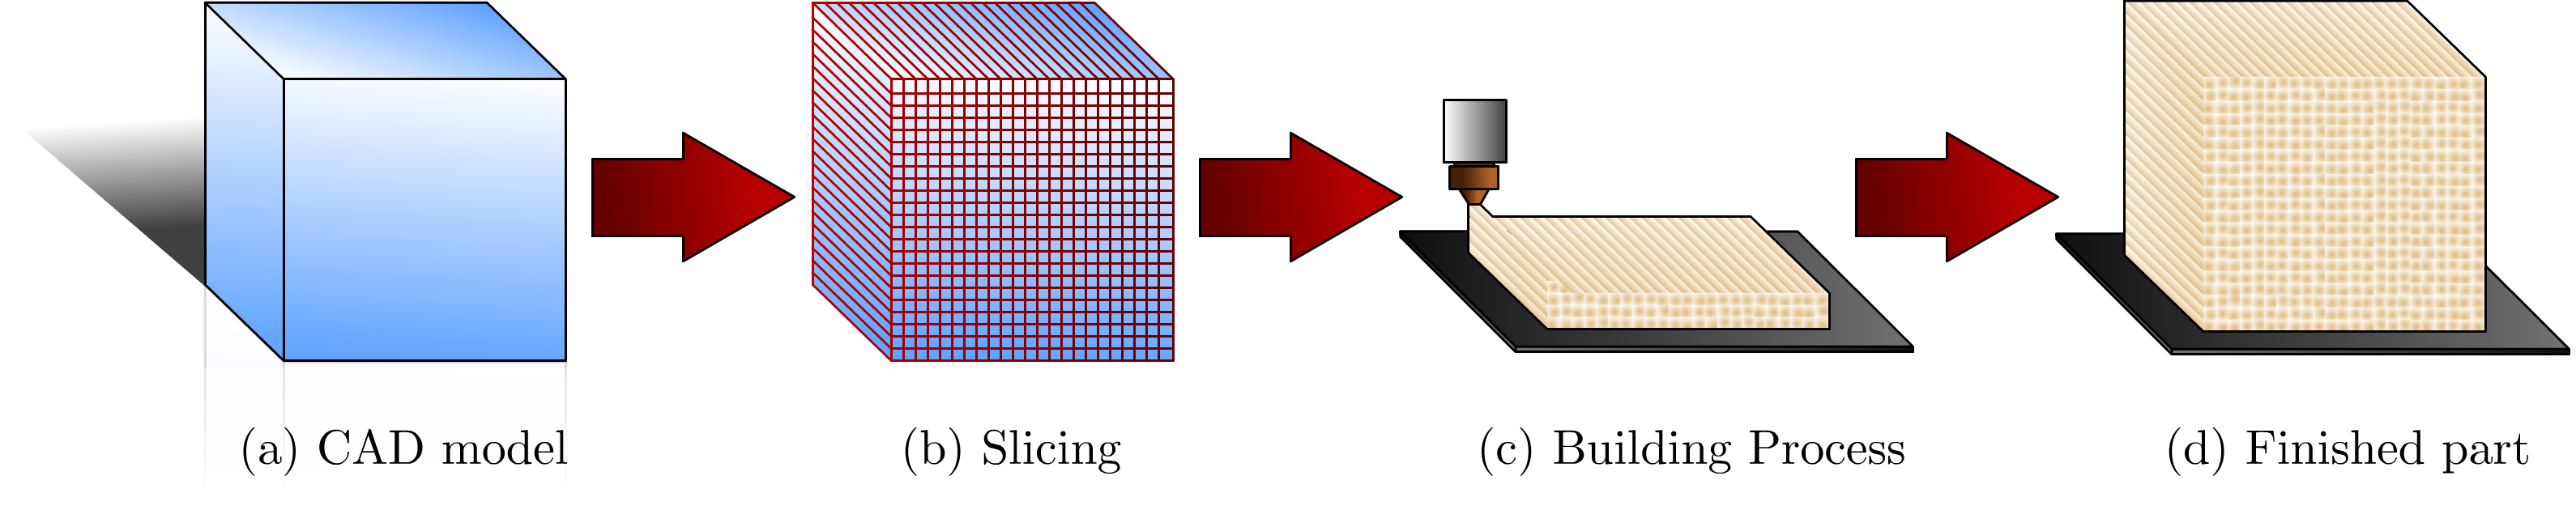
\includegraphics[width=\linewidth]{AM_flowchart_1}
	\caption{Process flow of AM} \label{fig:AM_flow}
\end{figure}
\pagebreak %Used to move the entire paragraph to a new page.
 
While all AM technologies operate on the same basic process flow described above, the specifics of each AM technique vary substantially, ranging from processes that use paper and binder, all the way through metal-based, laser tracing technologies. Since this is a rapidly evolving field, no general consensus exists for classifying the multiple AM processes available. However, the classification system proposed under the ASTM/ISO 52900 standard \cite{ASTM52900}, has been somewhat accepted by the field and divides AM technologies as follows:
\begin{enumerate}
	\item \textbf{Binder Jetting}: AM techniques where a binding agent is used to selectively promote cohesion in powder materials -generally gypsum, sand or metallic powders~\cite{ASTM52900,3DHubs2018}.
	\item \textbf{Directed Energy Deposition}: AM processes where a focused thermal energy source (i.e. laser, electron beam, plasma arc) is used to fuse materials as they are being deposited in the build volume. Materials are almost exclusively metals~\cite{ASTM52900,3DHubs2018}.
	\item \textbf{Material Extrusion}: In this type of AM technology, material is dispensed through a nozzle or orifice. Fused Filament Fabrication belongs to this classification. Materials are almost exclusively thermoplastics \cite{ASTM52900,3DHubs2018}.
	\item \textbf{Material Jetting}: AM techniques where build material is deposited selectively in droplets. Materials are usually wax or thermoplastics, but there are examples of metal-based, material jetting techniques \cite{ASTM52900,3DHubs2018}.
	\item \textbf{Powder Bed Fusion}: AM processes where portions of a powder bed are selectively fused through application of thermal energy. \emph{Selective Laser Sintering} (SLS) belongs to this category. Materials are usually thermoplastic polymers or metals \cite{ASTM52900,3DHubs2018}. 
	\item \textbf{Sheet Lamination}: In this type of AM technology, the final part is formed by bonding sheets of material -usually paper or composites \cite{ASTM52900,3DHubs2018}. 
	\item \textbf{Vat Photopolymerization}: In this AM process, a liquid photopolymer is selectively cured by a light source. \emph{Stereolithography} (SLA), arguably the first AM technology, belongs to this category. Due to the nature of this technique, the only materials used are photopolymers \cite{ASTM52900,3DHubs2018}.
\end{enumerate} 

\subsection{Advantages, Disadvantages and Success Stories}\label{subsec:AMAdDis} 
Since AM processes allow a relatively direct conversion of a CAD model into a constructed object, they were originally exclusively used for prototype development. For this reason, they were initially classified as \textquotedblleft \emph{Rapid Prototyping}\textquotedblright~(RP) technologies. This terminology is still used today, however, it is being superseded by \emph{Additive Manufacturing} since its potential to become a proper fabrication technique exists \cite{Gibson2015}. However, while being capable of quickly jumping from part design to manufacturing is a great advantage, AM has its own set of drawbacks. Table \ref{tab:AM_AdDis} summarizes the most noteworthy set of advantages and disadvantages typical of most AM technologies.

\begin{table}[h]
	\centering
	\caption{Advantages and Disadvantages of Additive Manufacturing}
	\label{tab:AM_AdDis}
	\begin{tabu} to 0.95\textwidth {  X[c]  X[c] }
		\hline
		\textbf{Advantages} & \textbf{Disadvantages} \\ 
		\hline
		Faster product development cycles \cite{Gibson2015} & Part quality highly dependent on process parameters \cite{Gibson2015}\\
		%---------
		No additional tools needed for part fabrication\cite{Gibson2015}&  Stratified build generally results in anisotropic parts \cite{Gibson2015, Capote2017}\\
		%---------
		Cost effective for small batches of parts \cite{Baumers2016,Conner2014,Berman2012}&  Costly for production of more than hundreds of parts \cite{Baumers2016,Conner2014,Berman2012}\\
		\hline
	\end{tabu}
\end{table}   

Out of all the described advantages and disadvantages, the high anisotropy of AM parts is responsible for the slow embrace of AM in highly demanding engineering fields -such as the aerospace and automotive industries. The highly anisotropic mechanical behavior makes it extremely difficult to predict part failure, therefore, it can't be implemented in engineering applications where catastrophic failure is to be avoided at all costs. Even so, success stories of implementation of AM in industrial environments are abundant. Below is a number of relatively 
recent examples:

\begin{itemize}
	\item \textbf{Volkswagen Autoeuropa}: This automotive assembly plant implemented the use of FFF machines to manufacture tools, jigs and fixtures used in their assembly line. They now produce 93\% of the tools that were historically externally sourced, and have reportedly cut their tool development time and costs by 95\% and 91\% respectively \cite{deVries2017}.
	\item \textbf{General Electric}: GE is currently producing in Alabama a complex fuel nozzle injector for the LEAP jet engine, using powder based, metal AM. The complex geometry of this component could not be manufactured by any other manufacturing technique. The production plant is expected to have 50 AM machines producing 35,000 fuel nozzle injectors annually by 2020 \cite{GEAdditive2016}. 
	\item \textbf{Adidas and New Balance}: Both shoe companies have developed separate approaches to constructing highly optimized, 3D printed midsoles for high performance running sneakers. New Balance makes use of SLS technology to build the intricate geometry of their \textquotedblleft \emph{Zante Generate}\textquotedblright~sneaker, using powdered TPU elastomer as the parent material. The designed honeycomb structure of the midsole, combined with the flexible material used, are supposed to improve the comfort and support brought by the shoe \cite{NewBalance2016}. Adidas on the other hand chose to develop the \textquotedblleft \emph{AlphaEDGE 4D LTD}\textquotedblright~running shoe using the CLIP technology by Carbon3D. While the cell geometry in  the midsole is also supposed to bring performance and comfort improvements, the final ambition of Adidas is to perfect the technology to a point where a customer can simply go to a shoe store, have their feet scanned, and receive a fully customized shoe with a 3D printed midsole that fits their particular needs \cite{Matisons2015,Saunders2018}. In both cases, the geometry of the midsole can only be produce by AM. The intricate structures in the midsoles can be seen in Figure \ref{fig:AMshoes}.
		
\end{itemize}
\begin{figure}[h]
	\center
	\subfloat[New Balance Zante Generate~\cite{NewBalance2016}\label{fig:NBZG}]{%
		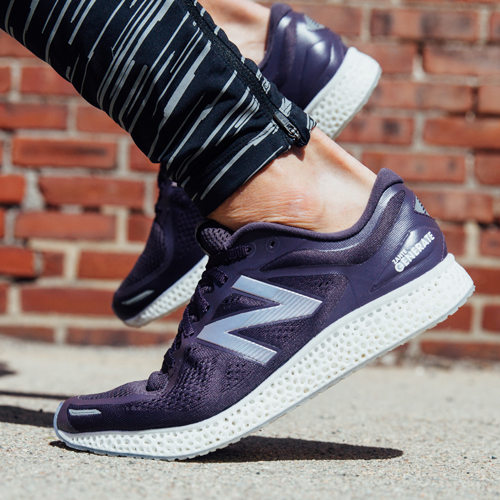
\includegraphics[height=6cm, keepaspectratio]{NB_generate}
	}
	\hfill
	\subfloat[Adidas AlphaEdge 4D LTD~\cite{Saunders2018}\label{fig:adidas}]{%
		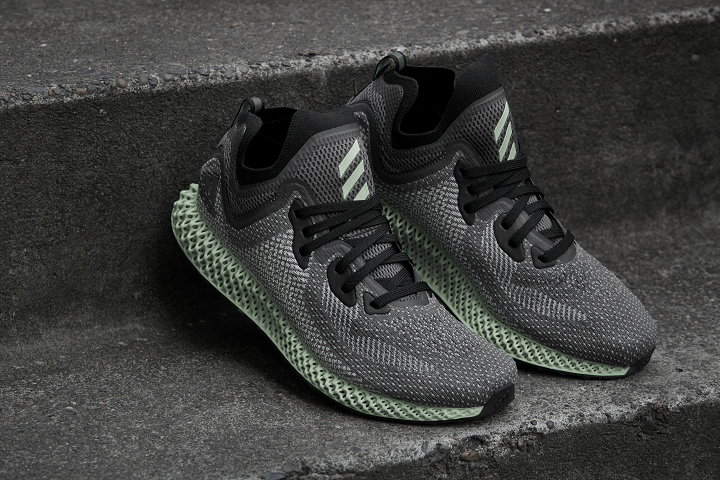
\includegraphics[height=6cm, keepaspectratio]{alphaedge_4D}
	}
	\caption{Shoes with AM midsoles}
	\label{fig:AMshoes}
\end{figure}

Note that in the cases presented, the main reason behind the usage of AM was either reduction expenses associated with producing small batches of parts, or the capability of reproducing a unique and complex geometry. This is a trend that is observed in most of the literature describing implementation of AM into industrial scenarios.

While the advantages and disadvantages described here cover the field of AM as a whole, each technique comes with its own set of pros and cons that may make it the preferred method to reproduce a particular product or geometry. This work, however, focuses solely on FFF. The specifics of this process are described in detail in Section~\ref{sec:FFF}.
\section{Fused Filament Fabrication}\label{sec:FFF} 
\emph{Fused Filament Fabrication}~(FFF) is an AM technology where the final geometry of the part is obtained through controlled extrusion of a liquid, self-hardening material -usually a thermoplastic polymer in molten state \cite{Gibson2015}. Originally developed by Stratasys in the 1980s under the \textendash~still trademarked \textendash~\emph{Fused Deposition Modeling}~(FDM\texttrademark) moniker, it has recently become one of the most widely used AM techniques due to the advent of low-cost, desktop FFF machines in the early 2010s caused by the expiration of key patents from Stratasys \cite{Gibson2015,Capote2017}. 

\pagebreak
\subsection{The FFF process}\label{ssec:FFFmach}

\begin{figure}[h]
	\center
	\subfloat[FFF printhead\label{fig:FFFnoz}]{%
		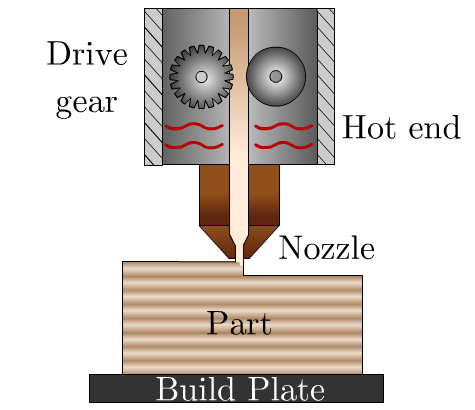
\includegraphics[height=6cm, keepaspectratio]{nozzle}
		}
	\hfill
	\subfloat[Typical FFF machine\label{fig:FFFmach}]{%
		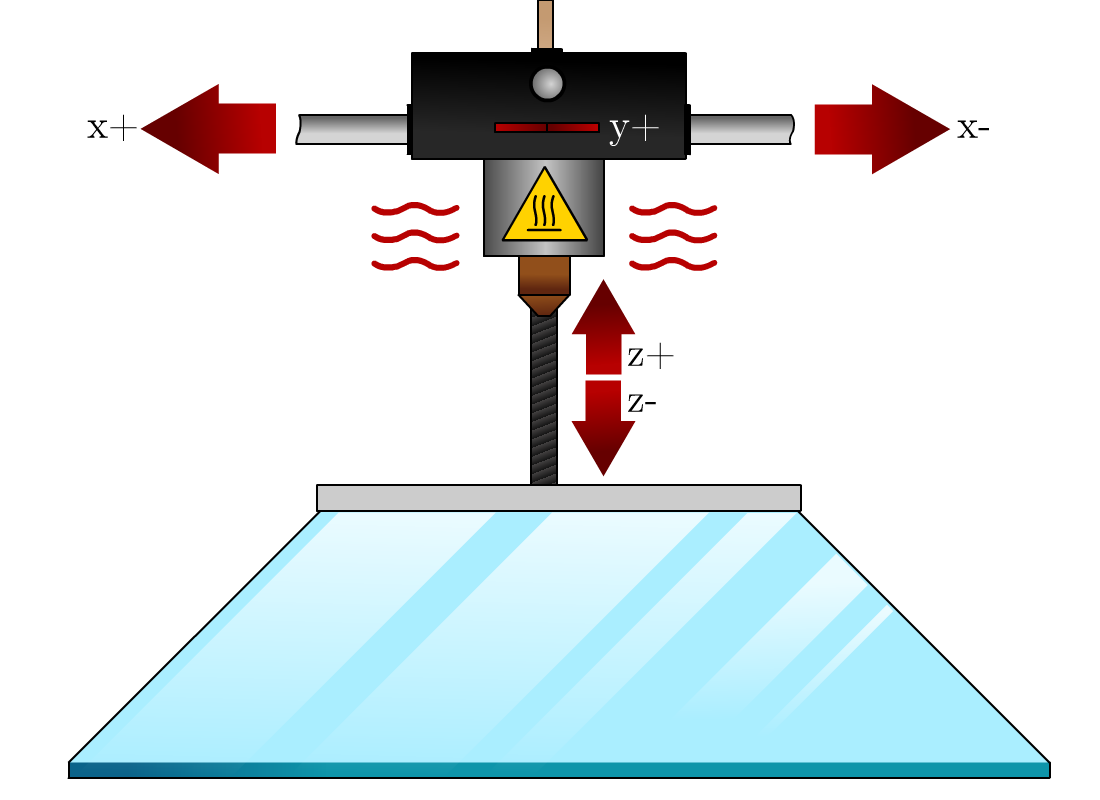
\includegraphics[height=6cm, keepaspectratio]{printer_layout}
		}
	\caption{The typical FFF machine configuration} \label{fig:machconfig}
\end{figure}
Like all AM technologies, the FFF process starts in a computer with a CAD model converted to the \emph{.stl} file format. The geometry is then translated to machine instructions through a \emph{slicing engine}, where the user inputs process parameters. Finally the \emph{toolpath} is executed by the FFF printer, building the object in a layer-by-layer basis -sometimes referred to as \emph{2.5D} printing. Figure \ref{fig:FFFflow} shows an abridged version of the process. The \emph{z} axis indicates the intended build direction. 
\begin{figure}[h]
	\center
	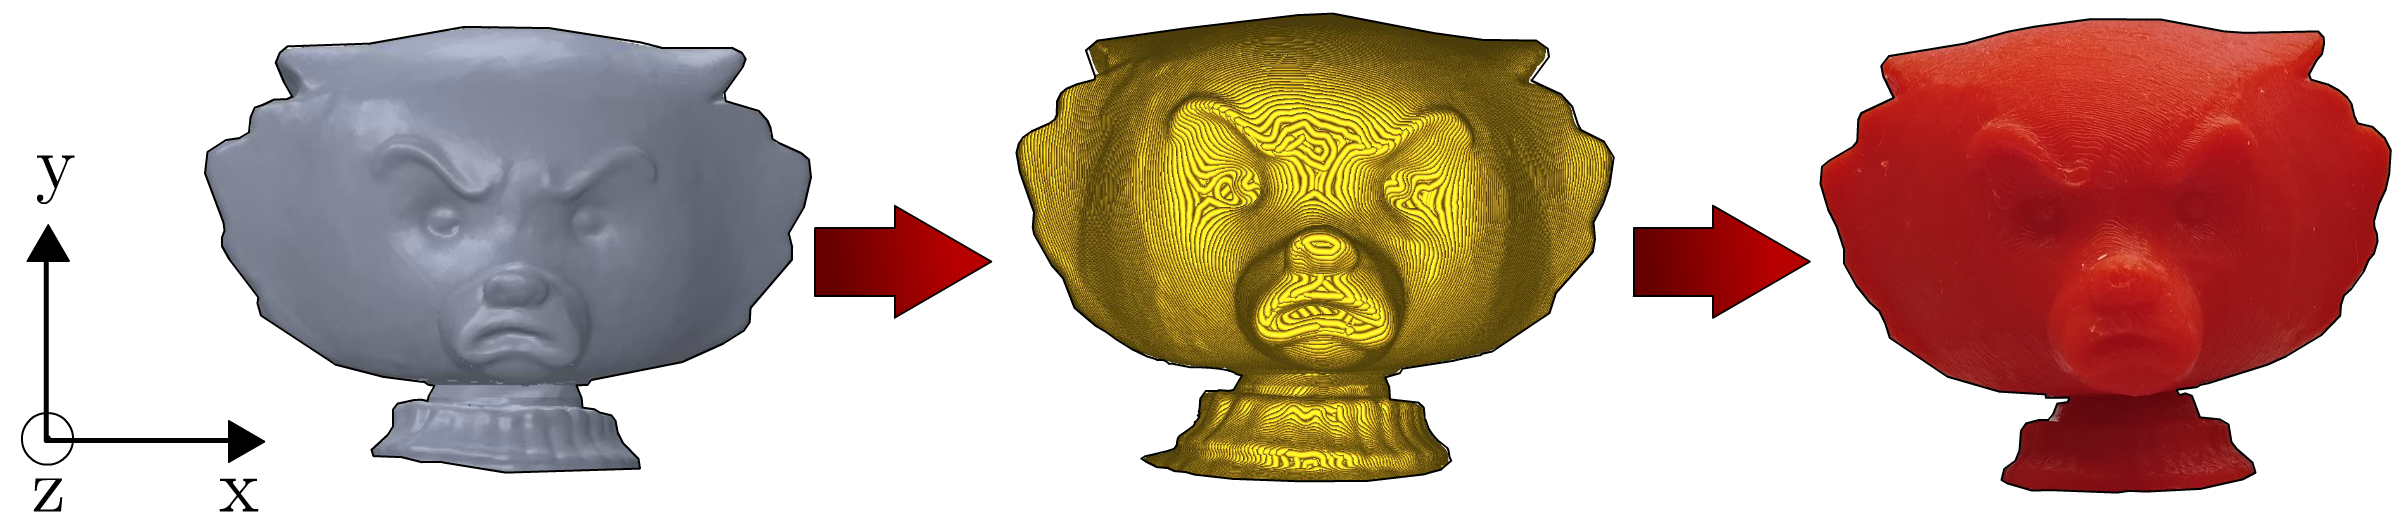
\includegraphics[width=0.95\textwidth]{FFF_flow}
	\caption{From left to right: stl, toolpath and final part} \label{fig:FFFflow}
\end{figure}
%Nomenclature introduced in this chapter:
\nomenclature[A]{SLA}{Stereolithography}% 
\nomenclature[A]{SLS}{Selective Laser Sintering}%
\end{document}
                %% machineConfigs.tex
% A discussion of possible machine configurations
\documentclass[main.tex]{subfiles}
\begin{document}
\chapter{Machine Configurations}
Deciding upon a machine configuration is just one of the many steps required to design and build a 3D printer.
This step is one which should be carefully considered since it is generally difficult to change the layout of a machine after construction.
The number of possible axis configurations is $n!$ and machine builders will create everyone of those combinations claiming it to be the best. 
To aid in choosing between machine configurations they can be broken down into three main categories: fixed build platform, fixed extruder, and moving build platform-moving extruder.
Additional comparisons will be made between systems with and without robotic arms.

\section{Number of Axes}
\label{sec:numberAxes}
In order to position a tool at any location and in any non-colliding posture on the outside of a convex part a minimum of five degrees of freedom are required.
Such machines are commonly referred to as five-axis machines and typically have three linear and two rotary axes.
The limitation of having only five axes to control a part with six degrees of freedom is that at some locations the tool can not move freely in any direction and may require a large reorientation to create an otherwise continuous tool path.
When using subtractive processing techniques such as machining, discontinuous tool paths add cycle time and may reduce the surface finish but the overall structural integrity and shape of the part is maintained.
However, for some additive processes such as automated fiber placement or continuous fiber 3D printing, discontinuous tool paths can greatly reduce the part's overall mechanical characteristics.
For these applications six axes are required with the 6R robots used in factory automation being one example.

Each additional axis used increases the cost, programming difficulty, and positioning inaccuracy for that machine.
Because of this, the decision to go beyond fives axes should be carefully considered.
The main advantage of six axes over five is preventing the machine from needing to be re-oriented during a continuous tool path.
An example re-orientation discontinuity occurs when a turn is made at the singularity of a rotary trunnion table, Fig.~\ref{fig:trunnion}.
For such a tool path the C-axis would need to rotate \ang{90} at the peak of the part.
Although this path is not ideal it would not negatively affect a traditional FFF printer. The extruder would pause, the table rotate, then the extruder would continue, without breaking the bead.
For automated fiber placement such a motion is not practical since it would cause tape buckling due to the a tight corner.
It is in general unlikely that there would be a need for such sharp turns in a tool path.
A square corner on a part will require a \ang{90} re-orientation to keep the nozzle normal to the part's surfaces no matter the number of axes on the machine and curved features tend to work best with curved tool paths.

\begin{figure}
\begin{center}
	\begin{overpic}[height=8cm, keepaspectratio]
		{TrunionMachine.pdf}
		\put(5,53){\textbf{C}}
		\put(68,47){\textbf{B}}
		\put(36,95){\textbf{Z}}
		\put(64,89){\textbf{Y}}
		\put(48,82){\textbf{X}}
		\put(8,65.5){\makebox(0,0)[r]{\small Tool Path}}
		\put(19,77){\makebox(0,0)[r]{\small Singular Point}}
	\end{overpic}
	\caption{Axis naming \cite{ISO841} and singular tool path.}
	\label{fig:trunnion}
\end{center}
\end{figure}

Due to the increased cost and programming complexity combined with the reduced precision, a traditional 3-axis machine having linear X, Y, Z axes combined with a two axis rotary table is the ideal working platform for off-axis printing.
With such a configuration all sides of the part not blocked by the build platform can be reached and every location can be reached at any configuration.
Programming is simplified when the rotary axes are used only for positioning and the actual printing is done in traditional 2.5D style.
This technique is called 3+2 since only the three linear axes are used while printing leaving the two rotary axes to be used only during orientation positioning.
Besides being easier to program, the 3+2 approach is typically more accurate since only three axes needs to be coordinated by the machine during printing.

Having a mature, robust, and off-the-shelf solution is most likely the number one reason 6R robots are often used in the off-axis 3D printing community \cite{Hedges2014, Arevo2015, Vurpillat2016}. 
These robots are designed for the demands of factory automation making them fast, accurate, and reliable.
They usually come with their own programming languages and simulation environments making them moderately easy to control and have the necessary hardware to interface with the print head.
When using robots large parts can be printed with a relatively compact machine, however there are limitations to this configuration which will be discussed later in this chapter.

\section{Fixed Build Platform}
Robotic configurations with fixed build platforms allow for the largest print volumes.
These robots can easily reach parts that occupy one quarter of their working volume and can handle even larger parts if the shape allows.
For extra long parts these robots can be mounted on rails and print parts of unlimited lengths.
Arevo Labs and the result of a collaboration between Lockheed Martin and Wolf Robotics are examples of this style of machine \cite{Hedges2014, Arevo2015}.
Due to the large surface area these machines can cover the build platform is often not heated so additional measures are needed to ensure proper bed adhesion.
With the nozzle mounted on the robot it is possible to decrease build times while increasing surface finish by keeping the head normal to the finished surface; however, there are limitations as to how steep of a surface material will adhere and not droop.
Having a fixed build platform does not enable the reduction of support structure.

\section{Fixed Extruder}
Using a fixed extruder with a robot mounted build platform does reduce the size of parts which can be printed but greatly increases the flexibility of both the tool path and the print order.
Parts can be finished with the nozzle normal to the exterior surface, as can be done with a robot held extruder configuration, but without any angle limitations.
Being able to rotate the part freely in space allows printed surfaces to be rotated normal to gravity reducing the need for support material.
This free rotation also enables printing across the traditional 2.5D layers created at the start of a part greatly decreasing its $z$ direction anisotropy.

As parts become larger both the part and the platform needed to hold it start to cause interference problems while printing with a robot held build platform.
With a robot mounted extruder the robot's payload is constant no matter how large the part, assuming the feed material is mounted separately.
With a robot held build platform this is not the case. 
As the work piece becomes larger the robot needs to hold and move more mass.
The build platform itself must be large enough to hold the work piece and adds considerable weight.
Large build platforms also make clearances with the extruder more challenging causing some of the flexibility created by this configuration to be lost when working towards the middle of the platform.

Song et al. \cite{Song2015} provide an interesting effort to produce a low cost six axis FFF printer.
In their design the extruder is mounted to a Gough-Stewart mechanism, a tilting platform moved by six linear actuators, with a fixed build platform underneath.
Their design provides full six axis motion enabling in plane finishing and contoured tool paths at a total cost of just over \$1400.
Although this design does provide a full six degrees of freedom, the max angles and work envelope are fairly limited.
With a tool angle of \SI{10}{\degree} about the $x$\nobreakdash-axis the working volume is about \SI{100}{\mm} x \SI{100}{\mm} x \SI{70}{\mm}, with additional limitations inside that range.
Even with these limitations it is an interesting machine which could be useful for home users who wish to increase the surface finish and strength of many of their parts.

\section{Moving Platform and Extruder}
The ideal configuration for flexible, off-axis 3D printing is an extruder which moves in X, Y, and Z, mounted over a trunnion table.
This configuration enables easy programming when performing 3+2 work, the trunnion table can be located in an arbitrary position and then G-code from standard slicing software could be used to print features in that orientation.
Having the axes on two separate platforms allows for more rigid and accurate construction when compared to a 6R robot since the positioning errors are no longer compounding in series.
A trunnion table will not allow parts as large as a robot held extruder configuration but tables with one meter swing diameters are commonly available%
\footnote{Nikken \SI{1200}{mm} trunion table: http://www.nikken-world.com/Nikken-5AX-1200-Ultra-Heavy-Duty.aspx}%
.

An excellent example of this style of off-axis printer and the advantages is can create was developed and tested at Mitsubishi Electric Research Laboratories \cite{Yerazunis2016}.
Their machine uses an in-house made tip/tilt trunnion table mounted under a delta printer providing five degrees of freedom.
By utilizing this machine configuration they are able to reach a larger portion of their build volume at a wider range of angles than is possible with Song's Gough-Stewart machine and it does not have the added complexity of a 6R robot.
By using a Bowden extruder their print head is kept light and the delta configuration for the $xyz$ motion of the print head provides an easier method for moving the head in three directions than a more typical Cartesian system.
Their tests on a printed dome specimen showed that the tool paths enabled by off-axis printing can create parts which are nearly 4.5 times stronger than that of a traditional FFF part.


Stratasys released a style of FFF machine at IMTS 2016, which they are calling ``3D Demonstrator'', that uses a two axis rotary table holding the build platform and a 6R robot holding the print head \cite{Vurpillat2016}.
Having eight axes creates a redundant system in their task space which can make programming much more difficult.
To reduce this difficulty they have chosen to always keep the tool aligned with the Z-axis, effectively simulating a three axis machine mounted over a trunnion.
Since the printing volume is limited to the space over the trunnion table only a small percentage of the robot's working envelope is used creating a system that occupies a much larger foot print than needed.

\section{Review}
Which type of machine configuration to choose depends on the particular applications for which it will be used.
For large parts which require minimal off-axis work a 6R robot with a fixed build platform and robot held print head is most likely the best choice.
When parts have tool paths with large off-axis angles then a moving platform will be required.
If an off-the-shelf solutions is desirable then an industrial robot is currently the best solution.
When more accuracy is desired or if work is being done to produce a better off-axis solution then a trunnion table with a moving print head should be explored.
For multi-material prints it will be tough to beat the ease of a robot held build platform with several fixed print heads mounted within the working range, see Table \ref{table:configcompare}.
Since the needs for this project were to print around a cylinder, i.e. steep off-axis angles, with the potential for multi-material prints, and without needing to create a new machine it was decided to use an industrial robot with a robot held build platform and a fixed extruder.

\begin{table}
	\caption{Optimal configuration based on application.}
	\centering
	\begin{tabular}{l l}
		\toprule
		\textbf{Application} & \textbf{Configuration} \\
		\midrule
		Large parts & Robot held extruder \\
		Multi-material & Robot held platform \\
		\addlinespace
		Steep off-axis angles & Rotating platform \\
		Off-the-shelf & Robot \\
		Increase accuracy & Trunnion table \\
		\addlinespace
		Reduced complexity & Five axes \\
		Avoid singular tool path & Six axes \\	
		\bottomrule		
	\end{tabular}	
	\label{table:configcompare}
\end{table}



\end{document}
                % % challenges
\documentclass[main.tex]{subfiles}
\begin{document}

\chapter{Challenges of Off-Axis 3D Printing}

Any system which moves from 2D to 3D experiences a dramatic increase in challenges, and 3D printing is no exception.
Although the name ``3D printing'' implies that the problem was already 3D, apart from computing the need for support structure the work is all done in 2D.
In standard 3D printing there is no need to worry about crashing the machine since the print head is either moving in the $xy$\nobreakdash-plane or is moving in the $+z$ direction away from the previously printed material.
This is not always true with off-axis printing.
For standard 3D printing the nozzle only needs to be accurately measured in the $z$ direction while the $x$ and $y$ directions can be approximated.
Not so for off-axis work.
Even choosing the correct order in which to print a part becomes ambiguous with off-axis printing.
For traditional printers, simply step up in $z$ and then print whatever needs to be there.
With off-axis printing the order in which features are printed is only limited by clearances and having a surface on which to print. 

\section{Reach, Clearance, and Collisions}
Since off-axis printing enables rotating the part out of the $xy$\nobreakdash-plane, it is now necessary to ensure collisions between the build platform, part, and print head do not occur.
Although finishing parts with the nozzle normal to the surface will provide the best surface finish, this will not be possible for all geometries.
In Figure~\ref{fig:nozzleCollision} it can be seen that the angle between the two features is too steep for the nozzle to clear the previously printed material.
If the surface finish on one of these features is determined to be more important than the other that feature could be printed first with the second feature printed in a typical 2.5D fashion.
If both features need a quality surface finish then one of the features could have its infill printed thick and then be finished in plane and then the other printed with low layer heights.
A solution not as fast as finishing both sides in plane but still faster than having to print everything with low layer heights.

\begin{figure}
\centering
	\begin{overpic}[height=8cm, keepaspectratio]
		{NozzleCollision.pdf}
		\put(100,85){Print Head}
		\put(95,62){Nozzle}
		\put(81,11){Printed Infill}
		\put(35,101){\makebox(0,0)[r]{Collision Point}}
	\end{overpic}
	\caption{Surface and nozzle geometry do not allow finishing part normal to surface.}%
	\label{fig:nozzleCollision}
\end{figure}

Without the ability for standard printers to print off-axis, nozzle designs up to now have not been optimized for these reach and clearance scenarios.
Work will need to be done to create a nozzle which is longer and skinnier enabling it to reach more locations.
Some nozzles may even need to be developed with angled orifices allowing them to print with the nozzle ``normal'' to the surface even with difficult to reach designs such as Figure~\ref{fig:nozzleCollision}.

\section{Bed Adhesion}
When performing standard 3D printing, warpage caused from differential cooling across layers creates forces which can break parts free from the print bed.
The majority of the print head's tool pressure is in the downward direction with only a small amount of lateral forces acting to remove the part from the print bed.
These lateral forces are small enough that only parts which have large height to adhesion surface area ratios tend to be affected with tall skinny parts occasionally becoming detached from the build platform causing a print to fail.
For off-axis printing the parts can now be rotated so that the downward force of the nozzle is no longer normal to the build plate.
These pressures can be larger than usual if there is overfilling of the part or the nozzle location is not properly calibrated, Fig.~\ref{fig:nozzleForces}.
This situation is made worse when small size build platforms are required in order to reach angled tool paths near the base of the part.
All of this may suggest that bed adhesion should be made high but there is an upper limit for adhesion since after printing the part needs to be removed without damage.
This implies that the adhesion between the first and second layers of the part must be higher than the adhesion between the first layer and the build platform.
The bonding between the part and the build platform could be aided by the use of releasable adhesives including hot-melt adhesives or electrically releasable adhesives \cite{Simon2010}.


\begin{figure}
\centering
	\begin{overpic}[height=8cm, keepaspectratio]
		{Bending.pdf}
		\put(3,36.5){\makebox(0,0)[r]{Part Deflection}}
		\put(-1,52){\makebox(0,0)[r]{Nozzle}}
		\put(76,51){\makebox(0,0)[r]{Increased Stress}}
		\put(76,66){\makebox(0,0)[r]{Build Platform}}
	\end{overpic}
	\caption{Nozzle inaccuracy increases stress at build platform.}%
	\label{fig:nozzleForces}
\end{figure}


\section{Joint Weakness}
Between layer adhesion is already a cause of weakness and warpage in 3D printed parts and this problem will continue in off-axis 3D printing.
It has been shown that layer print time and more specifically layer cooling have a major affect on how well consecutive layers adhere to each other \cite{Sun2015}.
If the previously printed layer has cooled below a critical temperature before the next layer is applied the bonding between the two layers will be weak often leading to cracking and warping of the part.
These failures typically happen on large prints or when multiple parts are printed at the same time since these scenarios increase the time between between layers.

For off-axis printing this between-layer weakness will cause problems at the joints where new orientations are printed across previously printed layers.
In many scenarios this joint will be located at the base of a new feature creating weak bonding at the location which experiences the greatest bending moments.
Special care will need to be taken when designing parts and tool paths to ensure that such joints are located in areas with lower stresses or have been made large enough to withstand the operating forces.

Since these joints will often be located in areas of high bending moments additional work should be done investigating techniques to increase their strength.
For example, it may be possible to design joints which create mechanical locking between beads instead of only relying on between bead adhesion.
Possible shapes could include dovetails, ball and socket, "Christmas Tree" groves used in turbines, or new shapes which are not manufacturable when using standard subtractive techniques but are possible for off-axis printers.

Localized re-heating could be another technique used to increase the strength of such joints.
Before layers of a new orientation are printed across cold base layers the part could be brought over to a heat source which warms the desired section above its critical adhesion temperature and create a bond equal in strength to a standard between layer interface.
This bond will not be as strong in tension as a continuous bead but will be much stronger than the bond created upon cold layers.

\section{Measuring Nozzle Location}
\label{sec:challangenozzle}
In 2.5D printing only the $z$\nobreakdash-height of the nozzle is critical, $x$ and~$y$ locations are relative to each other requiring the machine to only be repeatable, not accurate.
Should the $x$ and~$y$ locations be calibrated inaccurately, as long as the part is still printed on the build platform the accuracy is close enough.
Calibrating the $z$\nobreakdash-height is more critical but can be easily accomplished with a feeler gauge, often just a sheet of paper. 
When a part is printed with off-axis techniques the $x$ and~$y$ locations become as critical as the $z$ location.
If the $y$ location of the nozzle is not properly calibrated the part will be printed slightly shifted in the $y$\nobreakdash-axis.
Later when the part is rotated \ang{90} about the $x$\nobreakdash-axis to print beads across the layers the programmed $z$\nobreakdash-height will be incorrect causing beads to be printed too far from the part reducing their chance of adhesion or worse, the nozzle is too low causing it to collide with the part, Fig.~\ref{fig:locErrors}.

\begin{figure}
\centering
	\hspace{4pt}
	\begin{overpic}[scale=0.5]
		{Y_error_flat.pdf}
		\put(74,100){$x/y$ error ($\epsilon$)}
		\put(88,81){\shortstack[l]{Measured nozzle\\location}}
		\put(79,20){\shortstack[l]{Programmed\\location}}
		\put(10,17){\makebox(0,0)[r]{\shortstack[l]{Build\\plate}}}
		\put(17,34){\makebox(0,0)[r]{\shortstack[l]{Printed\\Location}}}
		\put(19,57){\makebox(0,0)[r]{Part}}
		\put(30,83){\makebox(0,0)[r]{\shortstack[l]{Actual nozzle\\location}}}
	\end{overpic}
	\hfill	
	\begin{overpic}[scale=0.5]
		{Y_error_horiz.pdf}
		\put(-1,60){\makebox(0,0)[r]{\shortstack[r]{Off-axis layer \\height error ($\epsilon$)}}}
	\end{overpic}
	\hspace{4pt}
	\caption{Location error in off-axis printing}
	\label{fig:locErrors}
\end{figure}

\section{Build Platform}
When working with 2.5D processes the table is designed to be as large as will fit in the machine.
With those processes a large platform provides more working space while producing very few drawbacks, namely some additional cost and weight.
For off-axis work a large platform can interfere with accessing features on the part which are at low angles near the build platform.
To minimize this interference it is best if the build platform is made as small as possible.
Instead of utilizing one large build platform, off-axis printers will need a variety of platforms varying in print area, distance from mounting surface, and angle from the 6th axis.
When performing off-axis operations a small set of platforms will generally cover a large percentage of the work but customized platforms will need to be developed from time to time for particularly difficult to reach tool paths.
It should be noted that it is not the part's geometry which dictates the build platform's geometry but instead the chosen tool path.
For a printer utilizing support structure any object which fits within its build volume can be printed utilizing 2.5D tool paths.
It is when off-axis printing techniques are used that the tool path will require clearance between the nozzle, part, and build platform.

\section{Tool Path Planning}
Of all the challenges in off-axis printing none is more difficult than tool path planning.
As work continues in anisotropic topology optimization new demands will be placed on the 3D printer to produce parts with not only difficult geometries but also specific bead orientations.
Creating such tool paths will not be easy and will require more input from the operator than current slicing packages enable.
Programs more similar to the CAM packages used in the machine tool industry will need to be created which allow a user to easily control how layers and regions are built.

Print order for 2.5D parts is set by $z$\nobreakdash-height and simply starts at the bottom of a part and works its way upward.
Off-axis printing does not suffer from this mandated print order.
This will provide it with the most opportunities to create higher quality parts, however, finding an optimum order in which regions of a part should be printed is a task analogous to the traveling salesman problem%
\footnote{The traveling salesman problem is a graph theory and optimization problem where, given a list of cities and the distances between them, determine the shortest possible route which visits each city exactly once and returns to the starting city.}
which, being an NP-hard problem, will be difficult to automate.
To handle the increasingly complex parts and design requirements demanded today, software will need to be developed which can use heuristics to properly weigh all of the design and process requirements and produce a tool path which is within an acceptable margin of the optimal solution.
These heuristics will combine hard limits such as machine reach and nozzle clearance with more flexible requirements including bead orientation, keeping beads continuous, amount of support structure, and surface finish.

\end{document}

                %% setup.tex

\documentclass[main.tex]{subfiles}
\begin{document}

\chapter{Equipment and Setup}

\begin{figure}
\centering
	\includegraphics[width=0.9\textwidth]{EnclosurePic.pdf}
	\caption{The robot in its enclosure holding an example part on the straight build platform with the angled platform on the table.}
	\label{fig:enclosurepic}
\end{figure}

\section{Equipment}
The following equipment was used for performing off-axis printing: an ABB IRB\nobreakdash-120 robot holding the build platform, a fixed LulzBot single extruder tool head v2, and a safety enclosure containing both the robot and print head, Fig.~\ref{fig:enclosurepic}.
A RAMBo motherboard located in a separate electrical enclosure, Fig.~\ref{fig:elecenclosure}, controls the print head and handles inputs from the robot.
In this print cell the robot is the master running the print motion program which controls the actions of the printer through digital I/O.

\begin{figure}
\centering
	\begin{overpic}[width=0.9\textwidth, keepaspectratio]
		{ElectricalEnclosure.jpg}
	\end{overpic}
	\caption{Electrical enclosure with RAMBo and power supply on the left and opto-couplers on the right. Some wires have been removed for clarity.}
	\label{fig:elecenclosure}
\end{figure}

\subsection{Robot}
An ABB IRB\nobreakdash-120 robot was chosen to be the platform to enable off-axis printing.
The style of the IRB\nobreakdash-120 is known as a 6R wrist-partitioned robot. 
6R means it has six rotary axes, as opposed to linear axes, and wrist-partitioned signifies that the robot's last three axes are in a ``wrist'' configuration signifying that all three of their axes of rotation intersect at a single point.
The robot has a \SI{580}{mm} reach, a max height of \SI{982}{mm}, and a max payload of about \SI{2}{kg} in the desired configurations.
The rated pose accuracy is \SI{20}{\micro m} with a pose repeatability of \SI{10}{\micro m}.

Although a 5\nobreakdash-axis trunnion table would be able to perform the required work, an industrial 6R robot was chosen since it provided an off-the-shelf solution that is mature and reliable, see Table \ref{table:configcompare} for configuration comparisons. 
With the robot's large work envelope it is possible to mount multiple extruders inside the safety enclosure enabling multi-material printing.

\subsection{Print Head}
A modified LulzBot TAZ single extruder tool head v2 is used for extruding the print material.
This head was chosen because experience with it on a Taz~5 FFF printer in our lab has shown it to be a reliable extruder.
It is an open source printer with models of the print head freely available making modifications easy to produce.
The stepper motor which drives the filament was moved to enable closer access to the nozzle.
In its factory configuration the stepper motor is normally mounted with the back of the motor extending out past the front of the extruder.
In this configuration a build platform rotated parallel to the $xz$\nobreakdash-plane can only reach to \SI{50}{mm} away from the centerline of the nozzle before contacting the stepper motor.
With the stepper motor switched to stick out the back side of the print head assembly the platform's minimum reach was reduced to \SI{20}{mm} away from the nozzle at which point the end of the large gear's axle contacts the platform.
Some modifications could be done to this axle to enable even closer reaches but they were not performed at this time.
Platforms with swing diameters less than \SI{50}{mm} can fit under the print head's framing and reach to within \SI{10}{mm} of the nozzle.
The small blower fan which cools the filament column was also moved to increase access to the nozzle.

To facilitate moving the stepper motor, a new extruder mount%
\footnote{http://download.lulzbot.com/TAZ/5.0/production\_parts/printed\_parts/extruder\_mount\_hex/}
was designed and printed.
The new mount has the stepper motor bolted behind the print head body and on the left side of the large herringbone gear.
Placing the motor on the left caused less interference with other hardware on the print head.
Glue was used to remount the small blower fan which cools the filament column above the heater also on the left side of the nozzle.
This side change was necessary because the large part cooling fan's location prevented moving the blower fan farther back on the extruder mount.

\begin{figure}
\linethickness{1pt}
\centering
	\subfloat[\label{fig:factoryhead}Factory Taz 5 print head.]{
		\begin{overpic}[width=0.55\textwidth, keepaspectratio]
			{Taz5Head_standard.JPG}
		\end{overpic}}
	\subfloat[\label{fig:modifiedhead}Modified print head.]{
		\begin{overpic}[width=0.4\textwidth, keepaspectratio]
			{PrintHeadQuartered.jpg}
			\put(8,30){\vector(2,3){10}}
			\put(-25,24){New stepper loc.}
			\put(40,15){\vector(5,1){16}}
			\put(39,15){\makebox(0,0)[r]{New blower loc.}}
		\end{overpic}}
	\caption{Stepper motor and small fan locations for factory and modified Taz 5 print heads.}
	\label{fig:printheads}
\end{figure}

\subsection{Print Head Controller - RAMBo}
A RAMBo motherboard is used to control the extruder stepper motor, two fans, nozzle heater, and bed heater.
The RAMBo board was designed by Ultimachine to be an open source plug and play hardware solution for RepRap 3D printers.
At its core is an Arduino Mega 2560 microcontroller with additional hardware integrated onto the PCB board for controlling a printer.
This hardware includes five stepper motor drivers, mosfets for controlling a print bed and two nozzles, internal resistors to create voltage dividers for the thermistors, plus many more connections for other printing hardware.
The board is powered with \SI{24}{\volt} DC power and can be programmed over USB.

When the RAMBo board is used to control a Taz printer it typically uses the open source Marlin firmware \cite{marlin2017}.
This firmware is designed to perform many different tasks, i.e. control up to five axes, monitor stroke limits, interpret G-code, etc., on a wide variety of machine configurations and platforms.
As such it is a moderately large and complex software set making modifications to the program difficult.
Since there are fewer tasks required of the RAMBo board with this off-axis application it was decided to write a program from scratch for controlling the print head instead of modifying the Marlin firmware.
This new program \cite{rambo2017} uses a state machine to control the extruder instead of a G-code interpreter allowing simple integration to the multi-channel digital I/O used for communication between the robot and RAMBo.

\section{Robot Print Head Interface}
\label{sec:interface}
Communication between the print head and robot is necessary to coordinate movements and increase print quality.
Without communication the print head or its program would need to know how long every robot positioning move would take in order for the extruder to start and stop extruding at the correct locations.
Multi-channel digit I/O was chosen as the communication method between the two systems.
Serial communication would be preferred but the option was not purchased with the robot and the addition of this communication layer was deemed too difficult to implement during initial setup of the system.
Outputs from the robot include when to start and stop printing and when to prime/retract the filament to prevent nozzle drool.
Nozzle and bed temperatures as well as extrusion rates are also sent from the robot to the RAMBo controller.
To transfer these values the RAMBo program is set into the appropriate state and then timed pulses are sent representing numeric values.
Inputs to the robot are currently limited to nozzle and build platform ``at temperature'' but may be expanded in the future.


The digital logic pins on the robot use \SI{24}{\volt} while the logic pins on the RAMBo board only use \SI{5}{\volt}.
Optocoupler relay boards were used to enable electrically isolated logic level stepping between the two systems.
A total of 16 inputs and 16 outputs are available on the robot and more than 32 pins are available on the RAMBo board.
Sixteen of the available RAMBo pins were originally designed for controlling an LCD screen and as such are conveniently located together on the board.
The remaining 16 pins will need to be scavenged from various other unused locations around the board.

\section{Setup}
When choosing the nozzle location and build platform design the following factors were considered:
avoiding robot singularities,
working envelope size,
robot to platform clearances,
and location of axis limits.
After balancing these factors a nozzle location and \ang{45} platform design was chosen with a second \ang{0} platform design being added later for producing continuous beads around cylindrical test specimens.


\subsection{Build Volume}
Creating a large build volume is a major goal when deciding upon nozzle location and build platform configuration.
Build volume is a simple parameter to characterize in 2.5D printers, simply multiply the travel limits of the three axes, but becomes more complex in off-axis printing.
When the robot is holding the platform at a fixed angle to the nozzle a large $xyz$\nobreakdash-space may be available.
At another angle only a small build volume may be reachable or the reachable build volume does not fully overlap the previous space.
The most permissive definition for build volume is thus the union of reachable work space for every platform angle.
Such a definition would provide a large build volume but some regions in this build volume would be work space singular meaning that at least one degree of freedom is lost in that region.
Because this union definition includes work space singularities a false impression is given as to the allowable part volume which can be printed utilizing off-axis techniques.

A more restrictive build volume definition could then be the intersection of reachable work space for every platform angle.
This definition seems to leave only the volume which can be reached at any angle however, due to the robot's axis limits combined with nozzle clearance problems, not every platform angle is reachable.
With unreachable angles the intersection would be an empty set, not a very useful value.
Eliminating unreachable angles still creates locations with infinitely small reachable volumes again creating an empty set.

A compromise was needed to balance the two previous definitions and provide a build volume that was a useful reference for design comparison.
The union definition contains too much volume that cannot provide the needed tool path flexibility while the intersection contains too many angles which would most likely not be required in a print.
The compromise was to define a \emph{cubic build volume} as follows: the volume of the largest cube whose five faces not touching the build platform can be printed with the nozzle normal to each face, Fig.~\ref{fig:buildvolume}.
A cube was chosen to make testing easier, requiring only five orientations be tested, and to eliminate the trade off between build volume and cross sectional area.
For example, some configurations may enable a cube of \SI{500}{mm} per side to be properly finished for a volume of \SI{0.125}{m^3} or a rectangular prism \SI{800}{mm} wide, \SI{200}{mm} deep and \SI{800}{mm} tall creating a build volume of \SI{0.128}{m^3}.
The later build volume is larger but the $xy$ aspect ratio is worse.
It cannot be said in general if the change in aspect ratio is acceptable since it may work for some parts and not others.
Similar problems can be found if a cylinder was used instead.
Choosing a cube eliminates the general problem of needing to know what aspect ratio is acceptable.

\begin{figure}
\centering
	\includegraphics[width=0.6\textwidth]{BuildVolume.pdf}
	\caption{A cube with side lengths of \SI{400}{mm} on Otto's angled build platform.}
	\label{fig:buildvolume}
\end{figure}

If a part fits inside the cubic build volume it is known that the part can be printed on the printer but tool path limitations may still exist.
These limitations are less likely to occur by requiring the faces of the cube to be printed while the nozzle is normal to them.
Disregarding part/nozzle interference problems, most parts which fit inside this build volume will be able to benefit from the off-axis printing goal of improving surface finish since each side of the part will be reachable with the nozzle normal to the surface.
The normal to cube face requirement also implies that large sections of the build volume are reachable at multiple angles enabling flexibility when creating continuous tool paths and printing without support structure.
Knowing if a specific tool path is achievable will require more detailed testing than simply checking cubic build volume but using this metric provides an easy method to compare platform configurations and helps show which part shapes are more likely to be reachable than others.


\section{Build Platform}
Two build platforms were designed and built for use on the robot.
The initial build platform was heated and had a build plate angled so as to be out of alignment from the sixth axis, Fig.~\ref{fig:angledplatform}.
While the angle of the platform enabled a large cubic build volume this configuration did not allow continuous beads to be printed around a cylinder.
Due to this limitation a new inline build platform was developed.

The inline platform, Figs.~\ref{fig:inlinepic} and~\ref{fig:inlinedrawing}, uses an aluminum base and an M5x0.8 stud onto which a semi-sacrificial ABS boss is threaded.
This ABS boss is the platform onto which parts are actually printed.
Since PLA sticks well enough to cold ABS there is no need to heat the build platform, see section~\ref{sec:bedadhesion} for more details.
During initial print tests the ABS platform would last for several parts before it would break during part removal.
Later parts were printed overlapping the ABS boss by \SI{3}{mm} which caused platform failures every time a part was removed.
Since these ABS pieces could be printed en masse on a traditional printer in less than \SI{10}{min/part} it was considered acceptable to use them as sacrificial pieces.
This platform design also allows flexibility when sizing the ABS boss eliminating nozzle clearance problems which occur when printing small parts on large platforms.
If a small part needs to be printed a small boss can be applied and vice versa.
Without the need for a heater this platform also prevented cable management problems which would have arisen when tool paths required turning the sixth axis multiple revolutions.

\begin{figure}
\centering
	\includegraphics[width=0.7\textwidth]{AngledPlatform.pdf}
	\caption{The original angled build platform.}
	\label{fig:angledplatform}
\end{figure}

\begin{figure}
\centering
	\begin{overpic}[width=0.9\textwidth, keepaspectratio]{MulticolorSpecimen.pdf}
	\put(61,36.5){\makebox(0,0)[r]{ABS boss}}
	\put(63,5){\makebox(0,0)[r]{Aluminum base}}
	\end{overpic}
	\caption{The inline build platform with a multi-colored specimen showing the grips in blue and gauge area in red.}
	\label{fig:inlinepic}
\end{figure}

\begin{figure}
\centering
	\includegraphics[width=0.9\textwidth]{InlinePlatform2.pdf}
	\caption{Drawing of the inline platform's aluminum base.}
	\label{fig:inlinedrawing}
\end{figure}

\subsection{Robot Enclosure}
The robot was mounted inside a safety enclosure to help prevent injuries during operation.
The enclosure is \SI{1200}{mm} (\SI{4}{ft}) by \SI{1800}{mm} (\SI{6}{ft}), large enough that with the robot mounted in the center and not holding a tool it cannot touch the sides.
Four polycarbonate paneled doors allow easy access to the robot for setup and convenient observation during operation.
Plastic coated wire fencing covers the two remaining openings.
The robot was mounted centered on the table, Fig.~\ref{fig:enclosuretop}, with the first axis's zero location splitting the enclosure into two nearly square sections.
From this location the robot can reach most of the enclosure allowing the maximum operating space.

\begin{figure}
\centering
        \includegraphics[scale=0.6]{Enclosure.pdf}
        \caption{Top view of robot enclosure}%
        \label{fig:enclosuretop}
\end{figure}

While this arrangement allows the robot to reach much of the enclosure it was later found to cause problems when using a build platform inline with the sixth axis.
The cubic build volume available with an inline platform is small, $\approx$ \SI{16}{cm^3}, for all nozzle locations as will be explained in section \ref{sec:accuracysolutions}.
6R robots such as the IRB-120 are most often used for pick and place applications and as such they are designed to have the most position and posture flexibility in the lower ranges of their reach.
Due to this intended design the robot position in the enclosure which would provide the largest build volume for off-axis printing using a platform inline with the sixth axis is actually upside down with the extruder at a $z$\nobreakdash-height near the base of the robot.
The IRB-120 is capable of being mounted upside down and with tool and work offsets the level of programming difficulty would remain the same.
An upside down configuration would require additional framing in the current enclosure design so it has not been switched but future projects should consider this mounting position.

\subsection{Singularities}
\label{sec:singularity}
The most common singularity encountered when operating a 6R wrist partitioned robot like the ABB IRB\nobreakdash-120 occurs when the 4th and~6th axes are parallel.
This parallel alignment is called a \emph{wrist-singularity} \cite{Hayes2002} and it removes one the robot's degrees of freedom preventing some tool postures and movement combinations from being achieved.
The two other singularity categories, shoulder and wrist singularities, typically only happen when the wrist is above the base and near the centerline of the first axis.
As long as the extruder is not placed directly over the robot these two singularities are typically avoided.

A common technique for avoiding a wrist singularity is to place the robot's end of arm (EOA)
\nomenclature[A]{EOA}{End Of Arm}
tooling at an angle to the 6th axis.
As the platform's angle becomes steeper the reachable build volume increases but it needs to be placed farther away from the 6th axis to prevent collisions between the platform and the 4th axis linkage.
Based on initial testing an angle of \ang{45} was chosen to be a good compromise between clearances and build volume, plus was a convenient number to help when checking position and posture values.
For the inline platform wrist singularities are avoided by printing the spiraled beads with the specimen angled \ang{45} away from the robot's $x$\nobreakdash-axis.

\subsection{Axis Limits}
One problem with the \ang{45} build platform is that continuous spirals around cylinders are not possible to produce.
The robot's 6th axis can rotate freely (the software limit is $\pm$242 revolutions) and the 5th axis has enough travel for the required moves, but to create a continuous spiral the 4th axis would also need to continuously rotate and its joint limitation is $\pm$\ang{160}.
This limitation requires that axes 4, 5, and 6 be reoriented once for each lap around a cylinder.
A simple technique for handling this reorientation is to only print half way around the part, reorient, and then print the other half.
Reorienting the part involves flipping axes 4 and 6 \ang{180} and changing the sign on axis~5. This reorientation places the work piece in the exact same location and posture as before but now the 4th axis can continue in the same direction as before with a fresh \ang{180} of travel available.

Reorienting the part half way through a pass causes two problems.
The first is the printed bead is no longer continuous creating print start and stop issues, surface irregularities, and potentially decreasing part strength.
The second problem is a limitation in the robot's accuracy.
The manufacturer's rated pose accuracy of \SI{20}{\micro m} is based on the ISO 9283  standard and is the difference between a taught position and positions obtained during program execution.
This implies that the robot will be in the same joint configuration when attempting to move to the desired location.
Tests have shown that when the $z$\nobreakdash-height of the robot is measured and then the end three axes are flipped the $z$\nobreakdash-height can change by almost \SI{300}{\micro m} and the measured nozzle location can change up to \SI{1}{mm}, Table \ref{tab:postionerror}.
With a minimum desired layer height of \SI{100}{\micro m} a minimum $z$\nobreakdash-height accuracy in the \SI{50}{\micro m} range is required with \SI{10}{\micro m} being preferred.
Accuracy in the $xy$\nobreakdash-plane is not as critical since the nozzle diameter is \SI{0.5}{mm} and the molten bead material can flow a little while being applied.
Since the pose error between the two robot configurations is much larger than the required accuracy additional measures need to be taken to enable accurate printing around a part.

\begin{table}
	\caption{Nozzle location error with axes 4, 5, and 6 flipped for one probe position.}
	\centering
	\begin{tabular}{r l}
		\toprule
		\textbf{Quaternion:} & 0.6533, 0.2706, 0.6533, -0.2706 \\
		\textbf{Robot Axes 1-3} (\si{\degree})\textbf{:} & -120, 7, -9 \\
		\bottomrule
	\end{tabular}
	\begin{tabular}{r c c c}
		\addlinespace
		& \multicolumn{3}{c}{\textbf{Robot Axes}\tablefootnote{Axis angles rounded to nearest degree to provide approximate robot configuration.} (\si{\degree})}\\ \cmidrule(r){2-4}
		\textbf{Pos. no.} & 4 & 5 & 6\\
		\midrule 
		1 & -90 & -75 &  91 \\
		2 & 90 & 75 & 271 \\
		\addlinespace
		& \multicolumn{3}{c}{\textbf{Coordinates} (\si{mm})} \\ \cmidrule(r){2-4}
		& X & Y & Z \\	
		1 & -21.00 & -433.50 & 636.96 \\
		2 & -21.82 & -434.04 & 636.69 \\ \cmidrule(r){2-4}
		Coordinate Differences & 0.82 & 0.54 & \textbf{0.27} \\
		\textbf{Abs. Position Difference:} & \textbf{1.02} & & \\		
		\bottomrule
	\end{tabular}
	\label{tab:postionerror}
\end{table}

\subsection{Pose Accuracy Solutions}
\label{sec:accuracysolutions}
Two possible solutions for the pose accuracy problem were considered.
Since the pose repeatability of the robot is within our desired tolerances the first solution considered was developing an accuracy map for the robot and then adjusting the programmed locations when calculating the tool path.
This technique is commonly done in industrial machines which have acceptable repeatability but less than desirable accuracy.
Lasers are typically used to create a volumetric accuracy map by placing a reflector on the EOA tooling and then having a fixed laser send/receive unit record the actual position of the reflector as the machine moves on a preprogrammed path.
This data is then used either directly by the robot or by the CAM software used to program the robot to adjust programmed positions enabling the robot more accurately position itself.

For the purposes of this problem a full accuracy map would not be necessary.
Since the current goal is to print around cylindrical parts the map would only need to be created at a few rotation locations around the desired path.
This map would then be imported into the tool path generation program which would adjust the commanded program positions to compensate for these errors.
This solution was not chosen since it increases the difficulty of tool path generation and still produces discontinuous beads.

The chosen solution was to redesign the build platform such that the sixth axis's center of rotation was normal to the print bed.
This allows torsion specimens to be printed with their central axis co-linear to the sixth axis.
With this configuration spiraled beads can be continuously printed around a cylinder simply by rotating the 6th axis while using axes 1-5 to move along the part's length.
This platform configuration keeps the robot in a small section of its joint ranges increasing movement accuracy and decreasing programming complexity since only axis six encounters a configuration change.
The large drawback of this configuration is the decrease in build volume.
With the chosen nozzle location the build height away from the platform is limited to $\approx$\SI{95}{mm} before the fifth axis reaches its joint limit.
Moving the nozzle higher or farther away from the robot can help this height limit but such a move greatly limits the working range when the part is rotated on its side for printing spirals.
Taking these limits together yields a cubic build volume of only \SI{16}{cm^3} which is a significant reduction in build volume when compared to the angle platform and limits the printable geometries considerably.
However, the desired tool paths for the test specimen all fall within the working range of this configuration making the inline platform a viable solution.

\subsection{Nozzle Location}
Nozzle location and build platform configuration must be designed together to ensure singularities and axes limits are avoided.
Based on initial work with the angled build platform it was found that a nozzle location \SI{430}{mm} away from the centerline of axis~1 and \SI{630}{mm} off the table enabled a cubic build volume of approximately \SI{400}{mm} per side or \SI{0.064}{m^3}.
This \SI{630}{mm} $z$\nobreakdash-height is the same as the robot's height in the home position (all axes at \ang{0}).
With the angled build platform axis six starts below the home position when the platform is just touching the nozzle and continues moving down as a part is printed taller.
If the nozzle was set in a higher position the robot would most likely have to move through a wrist singularity while printing a part since the sixth axis would have to transition from above the home position to below.

When using the inline build platform this chosen nozzle height can cause singularities while printing around a cylinder.
To prevent these singularities the part is rotated \ang{45} about the $z$\nobreakdash-axis when printing out of the $xy$\nobreakdash-plane.
Since the robot is using a robot held work object this \ang{45} rotation does not increase the programming complexity, it simply shifts the initial robot configuration.



\end{document}

                %% toolpath.tex

\documentclass[main.tex]{subfiles}
\begin{document}

\chapter{Robot Programming}
Two options are commonly available for programming most industrial robots: produce a standard G-code program and run it through the robot's G-code interpreter or use the robot's native programming language.
Using G-code is useful when the robot's tool paths will be generated by standard computer aided manufacturing (CAM) software packages.
\nomenclature[A]{CAM}{Computer Aided Manufacturing}
Most facilities with CNC machines already have access to CAM software and knowledgeable operators making it easy to transition from programming CNC machines to programming a robot.
CAM packages are also essential when tool paths require thousands to hundreds of thousands of points for complex machining or polishing applications.
There are, however, some disadvantages associated with using G-code on a robot.
The first disadvantage with G-code is that since it was originally designed for operating three axis CNC machines and only later expanded to handle more axes, it does not provide as rich of a command set for operating a robot as the robot's native language.
This can limit a programmer's ability to access robot specific reposition commands, handle advanced motion planning tasks, or interface with external devices.

A second disadvantage lies in needing to know the implementation and reliability of the robot's G-code interpreter.
Knowing which G-codes are implemented is usually simple but understanding the subtle differences which can occur between implementations can be difficult.
How will the robot move when G-code commands cause it to move near a singularity or require a different robot configuration to prevent a crash?
While these problems can also occur when using the robot's native language they become more opaque and difficult to predict with an additional layer of abstraction between the operator/programmer and the actual robot motions.

Due to the limitations present in using G-code to program the robot it was decided to use ABB's proprietary RAPID programming language for operating the robot.
By using the RAPID language it is possible to directly control the quaternions and robot configuration parameters for each point along a path making it easier to command off-axis work.
Communication between the robot and RAMBo board is easier with RAPID plus the RobotStudio environment simplifies program debugging.
For 2.5D printing it was possible to modify SciSlice to output RAPID programs instead of G-code enabling easy initial testing of the system.
When off-axis tool paths were required additional Python scripts were developed to produce the desired robot code.

When creating RAPID programs the most essential elements for making the robot move as desired are tool and work objects, motion commands, and the desired movement points.
The tool and work objects, sec. \ref{sec:toolworkobjects}, tell the robot where the tool and build platform are located providing a reference frame for the coordinate system.
Motions commands, sec. \ref{sec:motioncommands}, define how the robot should move between programmed points, i.e. straight line, arc, joint etc..
While points, or \texttt{robTarget}s, sec. \ref{sec:points}, define where the robot should move, what posture the tool should be in, and the desired robot configuration.
With these three basic items and knowledge of the robot's syntax, it is possible to create off-axis programs for the robot.



\section{Tool and Work Objects}
\label{sec:toolworkobjects}
As is done in CNC machine programming, tool and work offsets can and should be used when programming robots.
In ABB's RAPID programming language these offsets are stored in variable objects of types \texttt{tooldata} and \texttt{wobjdata}, respectively.
Unlike in CNC operations, the RAPID programming language allows a user to declare whether the robot is holding the tool or the work object.
Most applications use a robot held tool with a fixed work object but for this application it was decided to use a robot held work object (build platform) and a fixed tool (print head).
By using a robot held work object the $xyz$ coordinates used for commanding program positions become fixed to the part enabling the robot to track their locations as the part is rotated.
Calculating where the part is in space as the robot rotates, called the forward kinematics, is not overly complicated but it is work best completed by the robot itself.
With this setup a point on the part is always the same $xyz$ coordinates independent of the part's angle relative to the nozzle.
Commanding the robot to be at the same point with different orientations is done by using the same $xyz$ values and only changing the \texttt{robTarget}'s quaternion.
This makes it easy for the operator to know where on the part the robot is moving and which locations will have different orientations.
If a robot held tool and fixed work object had been used different positions around the part could be commanded with the same $xyz$ values but different quaternions, a situation deemed very difficult to read and troubleshoot.

Using tool and work objects also enables the operator to make adjustments to the tool path without editing and reloading the entire program.
If the operator notices that a new build platform was causing the initial layers of a part to be printed too high they could go into the work object representing the build platform and adjust it, fixing the tool path problem without changing the program.
It should be noted that in this situation the changing of the build platform made it obvious as to which object, tool or work, was causing the problem.
In other situations the adjustment required may not be so clear and special care should be taken when adjusting the location of the nozzle.
An adjustment in $z$\nobreakdash-height of the nozzle may fix a problem in the $xy$\nobreakdash-plane but create a new one when the work piece is rotated into a new orientation.

\subsection{Measuring the Nozzle}
As mentioned in section \ref{sec:challangenozzle}, accurately measuring the location of the nozzle in $xyz$ is critical to the quality of off-axis printed parts.
To measure the nozzle's location a 3-axis analog indicator made by Haimer, their Universal 3D-Sensor, was used which is accurate to \SI{10}{\micro m}.
A custom adapter was designed and then machined out of aluminum to attach the  3D-sensor to the robot, Fig.~\ref{fig:3Dsensor}.

\begin{figure}
\centering
	\begin{overpic}[width=0.8\textwidth, keepaspectratio]
		{3DSensor.pdf}
		\put(70,43){Robot Arm}
		\put(45,35){Adapter}
		\put(43,1.5){3D Sensor}
		\put(15,12){\makebox(0,0)[r]{Stylus on nozzle}}
	\end{overpic}
	\caption{Haimer 3D Sensor measuring nozzle location.}
	\label{fig:3Dsensor}
\end{figure}

\subsubsection{3D-Sensor Calibration}
Before making accurate measurements with the 3D-sensor the run-out of the tool must be minimized and the gauge length needs to be properly calibrated.
Run-out is minimized by adjusting the four run-out screws on the sensor and checked by rotating the sixth axis while the stylus is contacting a dial indicator.
With patience a run-out of less than \SI{2}{\micro m} can be achieved.

The gauge length of the sensor is measured from the mounting face of the sixth axis to the position of the stylus's tip when the dial reads zero in the $z$ direction.
To calibrate this value a reference location with a known $z$\nobreakdash-height must be developed.
This reference location was developed by commanding the sixth axis to be parallel with the safety enclosure's table and then driving the robot until a gauge block just fit between the table and the sixth axis's face.
From here the robot's $z$\nobreakdash-height is checked and by accounting for the height of the gauge block the $z$\nobreakdash-height of the reference position is known.
After the sensor is mounted on the robot and the run-out is adjusted the sixth axis is again placed parallel to the table and the robot is driven down until the 3D sensor reads zero.
The difference between the robot's $z$\nobreakdash-height in this position and that of the reference position is the gauge length of the tool.

\subsubsection{Measuring}
After properly calibrating the 3D sensor it is possible to begin measuring the $xyz$ location of the nozzle.
The flat end of the nozzle makes measuring its $z$\nobreakdash-height straight forward, drive the stylus into the nozzle until the reading is zero and record the $z$ value, but it is more difficult to measure the $xy$ location.
The technique used to measure the $xy$ location was to first drive the stylus into the nozzle until \SI{100}{\micro m} of deflection were observed.
Second the stylus was moved in the the desired direction until the ball started sliding off the flat face and \SI{10}{\micro m} of reduced deflection was observed, this $x$ or~$y$ location was recorded.
Third this process was repeated in the opposite direction with the appropriate location again being recorded.
Finally these two values were averaged to determine the center of the flat, Fig.~\ref{fig:nozzlemeasuring}.

\begin{figure}
\centering
        \begin{overpic}[width=0.7\textwidth, keepaspectratio]
        	{NozzleMeasure.pdf}
        	\put(18,5){\makebox(0,0)[r]{Step 2}}
        	\put(39,4){Step 3}
        	\put(49,45.5){Nozzle}
        	\put(79,62){\makebox(0,0)[c]{3D Sensor}}
        \end{overpic}
        \caption{Steps for measuring the $x$ or $y$ location of the nozzle.}%
        \label{fig:nozzlemeasuring}
\end{figure}

\begin{table}
\centering
	\caption{Nozzle location measurements}
    \begin{tabular}{r c c c c c}
    \toprule
    & \multicolumn{3}{c}{Nozzle Location (\si{mm})}\\ 
    \cmidrule(r){2-4}
    No. & X & Y & Z & Quaternion & Axis Angle\tablefootnote{Axis angles rounded to nearest degree to provide approximate robot configuration.} (\si{\degree})\\
    \midrule
    1 & -22.16 & -433.71 & 636.59 & (0.27, 0.65, 0.27, -0.65) & (-66, 3, -4, 91, -68, 91)\\
    2 & -20.97 & -433.81 & 636.77 & (0.5, 0.5, 0.5, -0.5) & (95, -15, 12, -119, -6, 120)\\
    \addlinespace
    3 & -21.00 & -433.5 & 636.96 & (0.65, 0.27, 0.65, -0.27) & (-120, 7, -8, 90, -75, 91)\\
    4 & -21.82 & -434.04 & 636.69 & (0.65, 0.27, 0.65, -0.27) & (-120, 7, -9, 90, 75, 271)\\
    \addlinespace
    5 & -21.60 & -433.38 & 636.81 & (0.65, 0.27, 0.27, -0.65) & (-94, -3, 29, -3, -70, 4)\\
    6 & -21.24 & -433.35 & 636.91 & (0.71, 0, 0.5, -0.5) & (-117, 13, 4, -59, -91, 36)\\
    7 & -21.87 & -433.41 & 636.79 & (0.5, 0.5, 0, -0.71) & (-69, 9, 8, 57, -86, -32)\\
    \midrule
    & 0.40 & 0.23 & 0.11 & \multicolumn{1}{l}{Standard Deviation} \\
    \cmidrule(r){2-5}
    & -21.52 & -433.60 & 636.79 & \multicolumn{1}{l}{Average} \\
    \bottomrule    
    \end{tabular}        
        \label{table:nozzlemeasurements}
\end{table}

To quantify and potentially compensate for pose inaccuracies the measuring procedure was repeated for seven different robot poses, Table \ref{table:nozzlemeasurements}.
Considerable variations were found in the $x$ and~$y$ directions which were caused by a combination of measuring difficulty and pose inaccuracy.
The $z$\nobreakdash-height is the most critical of the three dimensions and shows the least variation between measurements.
The averages of these values were used for the nozzle's tool data.

After performing several test prints it was found that the $z$\nobreakdash-height of the nozzle was \SIrange{200}{300}{\micro m} too low both when the platform was normal to the nozzle and when it was rotated to print around the outside of the part.
Placing the 3D sensor back on the robot provided numbers which showed that the entered $z$\nobreakdash-height was correct.
Additional testing revealed that the combined mass of the 3D sensor and adapter, \SI{680}{g}, cause the robot to deflect downward by \SI{250}{\micro m}.
Since the inline build platform has a mass of only \SI{72}{g} it does not deflect the robot down as far thus making the nozzle too close to the print.
Upon discovering this deflection the $z$ location of the nozzle was moved upward by \SI{250}{\micro m} fixing the $z$\nobreakdash-height problem.

\subsection{Measuring the Build Platform}
Measuring of the build platform was only necessary for the \ang{45} platform.
The inline platform, being a much simpler design, could be measured offline and its data manually entered.
When measured offline only the distance from the sixth axis's mounting face to the end of the platform is needed to set the $z$ value, both the $x$ and~$y$ values are set to zero and the orientation quaternion is set to $(0,-1,0,0)$ which signifies that the $z$ direction of the platform is straight away from the sixth axis.

Due to the difficulty in using offline techniques to measure the angled build platform it must be measured when attached to the robot.
Because of the platform's size and inaccuracies in manufacturing and assembly, both the location and angle of the platform relative to the sixth axis must be known to ensure proper nozzle heights when printing a part's first layer.
The robot provides a calibration routine which uses three measured points to automatically calculate the work object's distance and quaternion offsets from the sixth axis.

A modified tool setter was used to measure the three points needed for calibrating the angled build platform's work offset.
The tool setter is a Precise Dial Z-Axis Setter, no.~4401-0063, which had its original steel body replaced with a FFF printed ABS body to reduce its weight.
The weight reduction had been done to enable more precise print bed leveling on a standard 2.5D printer in the lab but was a useful modification here as well preventing additional deflection of the robot while measuring the work object.
When measuring the build platform the robot is first moved until the platform is under and approximately normal to the nozzle.
Next the tool setter is calibrated to a height of \SI{50}{mm} with a caliper and placed on the build platform.
Three points are chosen near the edges of the platform to provide the most $z$\nobreakdash-height difference if the platform is not at the correct angular position.
To control the orientation of the work coordinate system the three points are chosen in the order shown in Figure~\ref{fig:bedcalibration} with the first two points aligned with the robot's $x$\nobreakdash-axis for easier machine operation.
At each of the three points the platform's height is adjusted until the tool setter reads \SI{50}{mm} between the nozzle and the platform.

\begin{figure}
\centering
        \begin{overpic}[width=0.7\textwidth, keepaspectratio]
        	{BedLevelOrder.pdf}
        	\put(5.5,45.5){Nozzle}
        	\put(39,58){Build Platform}
        	\put(71, 58){Robot Arm}
        	\put(50,4){\makebox(0,0)[c]{\large{Main Operator Door}}}
        	\put(40,20){\textbf{1}}
        	\put(40,40){\textbf{2}}
        	\put(23,20){\textbf{3}}
        \end{overpic}
        \caption{Top view of platform showing order and location of work object calibration points.}%
        \label{fig:bedcalibration}
\end{figure}

After the calibration data is loaded into the work object the robot is commanded to move normal to and \SI{50}{mm} away from the nozzle.
The tool setter is then placed back on the platform and the calibration is checked.
Tests showed a total indicator runout, TIR, of only \SI{40}{\micro m}, within the flatness tolerance of the build plate itself.
\nomenclature[A]{TIR}{Total Indicator Runout}

It should be noted that the robot needs to know the mass and moment of its EOA tooling to ensure the acceleration and jerk movement parameters do not cause axis overloads.
This parameter is stored in the \texttt{tooldata} object.
When a \texttt{workobj} has its \texttt{robheld} parameter set to true the robot will read the tool mass and moment data from the active tool and apply it to the work object.

\section{Robot Motion Commands}
\label{sec:motioncommands}
There are two main programming techniques for commanding the robot's motion.
The first technique directly commands the angle for each axis while the second technique provides a desired path and an ending \texttt{robTarget} enabling the robot to calculate its own axis angle commands for the desired motion.
The \texttt{moveAbsJ} command is used when programming with the first technique.
With this command the absolute joint angles and tool center point, TCP, velocity are specified.
\nomenclature[A]{TCP}{Tool Center Point}
Each joint then moves at a speed such that the TCP velocity is maintained and all joints simultaneously reach their end position.
While this technique enables precise control over the robot, it has several disadvantages that make it infeasible for most programming applications.
One of the disadvantages is that if straight line motion is required, many waypoints along the path need to be calculated and then commanded making the program quite long and difficult to read.
A second disadvantage of using the \texttt{moveAbsJ} command is that it cannot use work and tool objects requiring recalculation of the entire program if either object needs adjustment.

A more desirable programming technique for off-axis printing is to use one of several RAPID provided movement commands depending upon which type of motion, linear, circular, joint, etc., is desired.
With these movement commands a desired \texttt{robTarget} is programmed and the robot calculates the waypoints required to move the robot along the intended path to the end location.
This greatly reduces the number of programmed points required and declares to the operator what type of motion the robot will make.
There are several limitations the robot places on these commands to ensure unexpected moves are not made.
The first limitation is that a single motion command is not allowed to move an axis on the robot more than \ang{90}.
This limitation is typically encountered when repositioning a print and not during normal printing paths.

The second limitation is the motion commands must avoid singularities, sec.~\ref{sec:singularity}.
During a singularity it is ambiguous as to which axis should move and how far.
For example, when a wrist singularity is encountered both the fourth and sixth axes cause motion about the same axis of rotation.
Instead of leaving the programmer/operator unable to know which axis the robot will choose to rotate, the robot instead sends an alarm and stops.
Moves which create singularities or cause axis over travel alarms are not checked for at program load time but are instead checked at runtime.
Simulation software such as RobotStudio or other third party software can be used to execute programs and check for execution time errors before they are encountered on the robot.

\section{Coordinates/Points}
\label{sec:points}
Coordinates are stored in RAPID as data of type \texttt{robTarget}.
\texttt{robTarget}s store three pieces of information about the point they represent: $xyz$ location, orientation quaternion, and the desired configuration of the robot, \texttt{robConfig}.
The $xyz$ location is in standard Euclidean space and is referenced from the active tool and work objects.
The quaternion used for controlling orientation represents the three rotational degrees of freedom with four numbers and must have a norm of one.
%Using four values in quaternions prevents representation singularities from occurring as can happen when using Euler angles or other three value representations and is more compact than a 3x3 rotation matrix.
These two parameters fully constrain the location and orientation of the robot held object but do not fully constrain the robot's axes values since some locations and orientations can be achieved by different axis angle combinations.
To clarify which combination is desired \texttt{robConfig} defines the location of axes 1, 4, and 6 in units of quarter turns from zero.
Together, these three parameters define a point's location, orientation, and desired axes positions.  

\section{System Communication}
As mentioned in section \ref{sec:interface}, the robot and print head communicate through the RAMBo board over multi-channel digital I/O.
The \texttt{SetDO} command sets the digital outputs either high or low while the \texttt{WaitDI} command waits until the print bed and extruder are up to temperature.
When setting the numeric values of temperature and extrusion rate the \texttt{WaitTime} command is used.


\section{Process Flow}
The RAPID program contains both the robot motion commands and the print head commands.
When a print head command is executed in the program a digital output is triggered on the robot's IRC5 controller.
This signal goes into the RAMBo enclosure where it is stepped down from \SI{24}{V} to \SI{5}{V} by an opto-coupler and a relay.
The \SI{5}{V} signal is then read by the RAMBo board.
If the signal is received while the RAMBo program is in the appropriate state the corresponding action will occur.
These actions can include sending drive signals to the stepper motor or adjusting the PWM signal to the heaters.
\nomenclature[A]{PWM}{Pulse Width Modulation}
Temperature information for the nozzle and bed are measured by thermocouples and read by the RAMBo board providing closed loop control of these values.
Nozzle and bed ``at temperature'' signals are currently the only communication from the RAMBo board back to the robot controller, Fig.~\ref{fig:progflow}.

\begin{figure}
\centering
    \includegraphics[]{ProgFlow.tikz}
\caption{Flow of commands and information during program execution.}
\label{fig:progflow}
\end{figure}

\end{document}

                %% validation.tex

\documentclass[main.tex]{subfiles}
\begin{document}
\chapter{Validation}

\section{Extruder}
Knowing the volume of filament being extruded during printing is critical for part strength and quality.
Under-extrusion causes poor bead and layer adhesion reducing part solidity and strength while over-extrusion reduces surface quality and often leads to print failure.
Direct volumetric flow measurements are not currently possible on FFF printers causing most printers to the use open loop linear displacement of filament as their method for controlling extrusion amounts.
Due to variations in filament diameter, voids within the filament, and feed gear slippage, simple linear displacement creates challenges when trying to accurately control part solidity especially for parts with target solidities near 100\%.
Some work has been done to create closed loop control for filament extrusion \cite{Greeff2017} which can both measure slippage at the feed gear and filament width allowing for more accurate volumetric flow rates but such a system has not been implemented on this extruder.
Without closed loop control the only method available for controlling flow rates is to accurately calibrate the filament's rate of linear displacement and from that value calculate the resultant flow rates based on the filament's measured diameter.

To calibrate the extruder's feed rate an extrusion rate of \SI{25}{mm/min} was set and two marks were placed on the filament.
\SI{25}{mm/min} was chosen as the initial calibration speed because it is the calculated extrusion rate needed for a print speed of \SI{1800}{mm/min} and layer height of \SI{0.2}{mm}, the values which were used for printing all of the torsion specimens used in this study.
The first mark was placed several millimeters above the extruder's inlet to ensure the stepper motor had finished accelerating before the mark entered the extruder.
The second mark was placed \SI{50}{mm} away from the first mark.
With the extruder at the material's operating temperature extrusion was started.
When the first mark entered the extruder a timer was started and the time between the first and second marks entering the extruder was recorded.
This time was then compared to the expected \SI{2}{min} and adjustments were made to the RAMBo program until the experimental result matched the expected result.

After the initial test produced an error of less than 1\% it was repeated at \SI{12}{mm/min} and \SI{50}{mm/min} with the length of the former being left the same and the later doubled to keep the test at \SI{2}{min}.
Both of these tests produced errors of less than 1\% showing the extruder to be effectively calibrated for a wide range of extrusion rates.

\section{Test Specimen}
A cylindrical torsion test specimen was chosen to enable comparing the strength of off-axis printed parts to those produced through traditional 2.5D printing.
This sample was chosen because it would provide an application and shape where off-axis printing could out perform a 2.5D printer without being too complex to tool path and test.
Since an FFF printed ASTM D638 tensile specimen is strongest when the beads are printed inline with the tensile forces a 2.5D printer can already produce an optimum bead orientation for that test specimen.
More complex shapes which should perform better when manufactured on an off-axis printer would be more difficult to test than a cylindrical torsion specimen and are not currently possible to tool path.
A printed part subjected to torsion should be strongest when the beads which make up its gauge section are wrapped around the outside of the cylinder allowing them to be more inline with the load path than beads printed straight along the part's length.
It is currently possible to create this tool path for our off-axis system and is a bead orientation which cannot be produced on a 2.5D printer.

This sample shape was also chosen because future work with off-axis printing will include analysis of the Osswald-Osswald failure criterion and build upon previous tests in this area \cite{Obst2017}.
In this model the $\operatorname{\sigma_{11}-\tau_{12}}$ and $\operatorname{\sigma_{11}-\tau_{13}}$ interactions are easiest to measure with a test specimen which has a hollow core and multiple layers of \ang{45} spiraled beads.
Previous studies were not able to measure these interaction values because it was not possible to print specimens with spiraled beads.
With off-axis printing these specimens will be producible allowing for a full analysis of the Osswald-Osswald model.

The test specimen design thus chosen for the off-axis printer is a hollow cylinder with $\pm$\ang{45} spiraled beads.
It is not currently possible to print a sample with only spiraled beads since the first layer of the spiral would have no surface on which to rest while cooling.
Instead a central core must first be printed in traditional 2.5D fashion onto which the spiraled layers are printed.
Having an internal core not at $\pm$\ang{45} will the affect interaction value measurements and calculations, so the test specimens are designed to have a spiral thickness $10\times$ the thickness of the inner core.
Previous work had used a hollow torsion specimen with an inside diameter of \SI{7}{mm} so that value was also used as the outer diameter of the core.
This \SI{7}{mm} value is around the minimum diameter which can support the tool pressures encountered while printing the spirals so no attempts were made to print smaller cores.
Previous work had used a sample \SI{170}{mm} in length but, due to travel limitations of the 5th axis during core printing with the inline build platform, the specimen length was set to \SI{95}{mm} preventing axis over travel alarms, Fig.~\ref{fig:torsionspecimen}.
Future work will include printing a central core from PVA, a water soluble material, so that fewer spiraled layers need to be printed reducing the specimens diameter and print time.
These central cores can be printed on a different machine eliminating the \SI{95}{mm} height restriction.

\begin{figure}
        \includegraphics[width=0.9\textwidth]{twisttest.pdf}
        \caption{Torsion test specimen - (\si{mm})}%
        \label{fig:torsionspecimen}
\end{figure}

\subsection{Off-Axis Printing}
Printing of the off-axis test specimens starts with two 100\% infill circular layers printed on the build platform.
Printing these two complete layers first creates a larger surface contacting the print bed allowing for greater bed adhesion than just a spiraled core would be able to produce.
A larger contact area between the two surfaces helps prevent bed adhesion failures when starting the first spiraled layer, sec.~\ref{sec:bedadhesion}.
Next the inner core is printed as a continuous \SI{7}{mm} helix to a height of \SI{95}{mm}.
Both of these sections are printed with the build platform normal to the nozzle and with a layer height of \SI{0.2}{mm}.
By printing the inner core with a continuous helix instead of layer by layer the surface finish of the cylinder was greatly improved and the print time was decreased.
These improvements were possible because a continuous helix eliminates the stopping and starting which would normally occur at each layer.
Experiments done at different print speeds showed that single walled helix cylinders of any size printed with PLA at \SI{220}{\degreeCelsius} would produce failures if a lap around the helix took less than 1.8 seconds.
When lap times were below this value the previous layers would not cool enough causing them to buckle and produce cylinders with poor circularity and surface finish.
The \SI{7}{mm} cylinders where thus printed at \SI{10}{mm/sec} to prevent this problem.

After the inner core was printed the build platform was rotated to allow printing around the outside of the core at a speed of \SI{30}{mm/s}.
As previously mentioned the cylinder is placed rotated \ang{45} off the robot's $x$\nobreakdash-axis to prevent wrist singularities, sec.~\ref{sec:singularity}.
Every layer starts with the same side of the cylinder up, i.e. with the sixth axis at the rotation angle, and begins printing at the end of the core nearest the build platform.
By starting each layer with the sixth axis at the same angle some layering bias is created in the part.
This problem could be prevented by starting each layer at a random rotation angle but such code was not implemented.
From there the layers were printed from the bottom of the core to the top and back again repeating until the entire layer was finished.
By printing the beads back and forth from top to bottom instead of only from the bottom to the top it was possible to print each layer in one continuous path again improving surface finish and reducing cycle time by eliminating retractions.
To help prevent bed adhesion failures the 25 layers were printed beyond the interface between the print bed and the helix core allowing them to extend onto the outside of the build platform by \SI{0.5}{mm}.
After successfully printing multiple samples with this overlap distance prints began experiencing bed adhesion failures.
Re-performing the bed adhesion tests showed adhesion values approximately one quarter the original test results.
To prevent further bed adhesion failures the overlap distance was changed to \SI{3}{mm}.
At this distance it was not possible to remove parts from the build platform causing the platforms to be used as sacrificial parts instead of their previous use as a wear part.

After all 25 layers were finished the grips were printed onto the part.
The complete lower grip was printed first and then the upper grip was printed.
If the grips had been printed one layer from one, one layer from the other, nozzle drool would have caused stringing across the part each time the nozzle switched grips.
Printing one complete grip and then the other also allowed for each grip layer to be hotter when the next layer was printed helping to increase the strength between layers, Fig.~\ref{fig:offaxislayers}.
No cracking of the grips was observed during testing showing that there was sufficient between layer adhesion in these areas.

\begin{figure}
\centering
	\begin{overpic}[width=0.4\textwidth, keepaspectratio, angle=90]
		{Otto_Torsion.pdf}
		\put(18,35){\makebox(0,0)[r]{Helix core}}
		\put(29,39){25 layers $\pm$\ang{45}}
		\put(58,39){Grip}
		\put(74,31){A}
		\put(74,0){A}
	\end{overpic}
	\caption{Layers in off-axis printed samples. Not to scale.}
	\label{fig:offaxislayers}
\end{figure}

When printing beads of material to cover a predefined area it often happens that an integer number of beads would either slightly under-fill or slightly overfill the space.
Most open source slicing software uses a fixed distance between adjacent beads, often called \emph{path width}, and fills the available area with beads this distance apart leaving a gap in any area where the next bead does not fit.
This option was not chosen for the torsion specimens since it would consistently leave gaps along the line where a layer starts and ends.
Instead it was chosen to provide a guideline value for the path width, the nozzle diameter of \SI{0.5}{mm}, and then dynamically adjust the actual path width for each layer based upon how many beads can evenly fit in the layer.
The dynamic allocation calculates the number of beads which will fit into a layer with the equation

\begin{equation}
n = \left[ \frac{c \times \sin(\theta_H)}{W} \right],
\end{equation}
where $n$ is the number of printed beads, the square brackets ``[ ]'' mean \emph{round to nearest integer}%
\footnote{This formula was implemented in Python which uses the IEEE 754 recommended round to nearest even integer for values halfway between two integers.}%
, $c$ is the finished circumference, $\theta_H$ is the helix angle, and $W$ is the desired path width.
\nomenclature[S]{$n$}{Number of beads \nomunit{-}}%
\nomenclature[S]{$c$}{Circumference \nomunit{\si{mm}}}%
\nomenclature[S]{$\theta_H$}{Helix angle \nomunit{\si{\degree}}}%
\nomenclature[S]{$W$}{Desired path width \nomunit{\si{mm}}}%
This number of beads is then evenly distributed across the current layer.
Since \emph{round nearest} was chosen to convert the decimal value into an integer instead of \emph{floor} a layer may become over or under filled.
To prevent problems associated with overfilling a max overfill value for a layer was set to 1\%.
Although this technique can lead to problems for areas with very few beads, even the first helix layer of the specimen, printed at a diameter of \SI{7.4}{mm}, with an angle of \ang{45}, needs a theoretical 32.8 beads which, when rounded to 33, produces an overfill of only 0.4\%.
For all 25 layers of the specimen, printed at a layer height of \SI{0.2}{mm}, only the 7th layer has its number of beads reduced from 44 to 43 with the 1\% max overfill rule.
The worst under-filling is on layer 3 at 1.2\%.
The average filling across all 25 layers is 0.04\% under-filled, considerably better than the extrusion volume accuracy.

\subsection{Standard 2.5D Printing}
2.5D printer comparison test specimens were printed on an Ultimaker 3 FFF printer.
The specimens were printed on their side with $\pm$\ang{45} infill and one shell, Fig.~\ref{fig:buildorientation}.
A layer height of \SI{0.2}{mm} was used to match that of the off-axis prints.
The Ultimaker 3 version of the open source Cura slicing software was used to generate the tool paths.
Due to the print geometry and orientation, support structure was required to create the print.
A PVA water soluble support material was used along with Cura's ``touching bed'' support structure option to create support material only on the outside of the part and not inside the hollow core.
Tests showed that the hollow core could be printed successfully without the use of support material.

\begin{figure}[!h]
\centering
	\begin{overpic}[width=0.8\textwidth, keepaspectratio]
		{buildorientation.pdf}
		\put(0,14){Z}
		\put(13.5,0){X}
	\end{overpic}
    \caption{Build orientation on 2.5D printer.}%
    \label{fig:buildorientation}
\end{figure}

\subsection{Material}
MatterHacker's \SI{3}{mm} diameter red PLA batch number 2016-09-12-1 filament was used in this study.
Both the off-axis samples and the comparison 2.5D printed specimens were manufactured from the same spool of filament for all of the tests eliminating any differences which often occur between filament production runs.

\subsection{Post Processing}
The test specimens created on the off-axis printer required additional machining to create flats on the grips.
These flats allowed the three jaw chucks on the torsion testing machine to more reliably hold the specimens.
To machine the flats the specimens were placed in a rotary indexing head and clamped in the indexing head's three jaw chuck on the central body of the specimen.
Clamping on the central body ensures the flats are positioned equidistant from the specimen's neutral axis.
The flats were machined the full length of the grip and to a depth such that the smallest flat was at least \SI{10}{mm} wide.
After three flats were machined into one grip the sample was flipped and three flats were machined into the opposite grip.
Since the torsion testing machine can start with the powered head at any angle no effort was made to index the flats between ends.

Specimens created on the standard 2.5D printer were soaked in \SI{55}{\degreeCelsius} water over night to soften the PVA support structure for removal.
These specimens were printed with flats on the grips to eliminate the machining step, however, the three $\pm$\ang{45} specimens warped at their grips and therefore did require machining.
The specimens were then dried overnight in desiccant to help mitigate any material property changes which may have occurred from their time in warm water.

\section{Bed Adhesion}
\label{sec:bedadhesion}
Bed adhesion tests were performed to determine how well the helix core stuck to various print bed materials.
These tests were necessary since the printing forces are not normal to the build platform as they are in 2.5D printing but instead will create bending moments on the helix core which can cause delamination from the print bed.
To perform the bed adhesion tests helix cores of 7, 10, and \SI{15}{mm} diameters and \SI{60}{mm} in height were printed and broken off.
Each core had two full layers printed at the base before the helix started.
After the core was printed it was rotated until it was parallel with the ground.
Next increasing amounts of weight were suspended from the core \SI{50}{mm} from the base until the core broke off the platform, Fig.~\ref{fig:bedadhesion}.
Each test was only performed with one sample and the weight at failure was recorded.
From these measurements the stress on the upper surface of the core can be calculated using equations \ref{eq:stress} and~\ref{eq:IxSolid}, with the results given in Table~\ref{tab:bedadhesion}.

\begin{table}
\caption{Stress on upper surface of PLA core at bed adhesion failure.}
\centering
\begin{tabular}{l c c c}
	\textbf{Bed Material} & \textbf{Core Diameter} (\si{mm}) &
		\textbf{Mass} (\si{g}) & \textbf{Stress} (\si{\mega\pascal}) \\
	\toprule
	ABS & 15 & 2290 & 3.4 \\
	ABS & 7 & 310 & 4.5 \\
	\midrule
	PLA & 15 & 1260 & 1.9 \\
	PLA & 10 & 240 & 1.2 \\
	PLA & 7 & 130 & 1.9 \\
	\midrule
	Heated AL & 15 & 180 &  0.27 \\
	Heated AL with Glue & 15 & 145 & 0.21 \\
	Heated AL with Tape & 15 & 95 & 0.14 \\
	\bottomrule
\end{tabular}
	\label{tab:bedadhesion}
\end{table}

\begin{wrapfigure}{R}{0.4\textwidth}
\centering
	\includegraphics[width=0.38\textwidth]{bedadhesion.pdf}
	\caption{A \SI{1}{kg} weight testing bed adhesion between PLA (left, blue) and red ABS (right red).\\}
	\label{fig:bedadhesion}
\end{wrapfigure}

Since only the first two layers of the core were solid and the rest of the layers had a \SI{0.5}{mm} wall thickness it was not known if the bending stress would be fully transferred to the solid base or only act upon an outer ring on the base.
Because of this unknown the stress calculations were done for both a hollow cylinder and a solid cylinder.
The equation for stress on the upper surface of a cantilevered cylinder is
\begin{equation}
\sigma = \frac{M_z r}{I_x}
\label{eq:stress}
\end{equation}
where $M_z$ is the bending moment, $r$ the radius, and $I_x$ the area moment of inertia.
For solid cylinders
\begin{equation}
I_x = \frac{\pi}{4}r^4
\label{eq:IxSolid}
\end{equation}
while for hollow cylinders
\begin{equation}
I_x = \frac{\pi}{4}\left(r_2^4-r_1^4\right)
\end{equation}
where $r_2$ and $r_1$ are the cylinder's outer and inner radii, respectively.%
\nomenclature[S]{$\sigma$}{Stress \nomunit{\si{Pa}}}%
\nomenclature[S]{$r$}{Radius \nomunit{\si{m}}}%
\nomenclature[S]{$I_x$}{Area moment of inertia \nomunit{\si{m^4}}}
It is expected that the stress at failure will be constant for each bed material and not vary relative to core diameter.
When comparing the two calculations the solid values, shown in Table \ref{tab:bedadhesion}, were found to be approximately the same for each bed material while the hollow tube values showed the \SI{7}{mm} cores to fail at a stress eight times larger than the \SI{15}{mm} cores.
Since the values obtained from the solid beam calculations aligned with the expected values it is assumed that the stress is well transferred from the thin helix section to the solid base layers thus making these values the more accurate approximation.

Only one test of each sample was performed so these results should not be seen to provide exact values but there is enough of a spread between different bed material data points to make a general conclusion.
The main conclusion to be made from these results is that PLA adheres best to an ABS build platform performing twice as well as PLA and a factor of ten better than an aluminum platform.
This result is slightly surprising since it had been assumed that PLA would bond best to itself.
Further tests should be done printing ABS onto an ABS platform to determine if ABS adheres best to itself or if the ABS/PLA combo is what provides the extra strength.

After performing these bed adhesion tests multiple specimens were successfully printed without experiencing bed adhesion failures.
Several weeks later bed adhesion problems began occurring on nearly every print.
Additional bed adhesion tests were then performed which showed adhesion strengths of approximately one quarter that of the previous tests.
Adjusting the $z$\nobreakdash-height and trying several ABS build platforms did not fix the problem.
Old successful platforms and new unused platforms were tested all showing similar low adhesion strengths.
Due to time restrictions more thorough tests were not able to be performed but it is suspected that increased humidity in the lab due to changes is weather is related to the problem.

Tests have not yet been performed to correlate initial $z$\nobreakdash-height with bed adhesion.
Anecdotal evidence from warpage on 2.5D printers seems to show that setting the first layer's $z$\nobreakdash-height too high increases the chance of warpage implying that printing the first layer too high also decreases bed adhesion.
Further tests should be performed to determine how accurately the $z$\nobreakdash-height needs to be set and how much it affects bed adhesion.

Tests have also not been performed which measure the tool forces during printing.
If this value was known it would then be possible to know how much bed adhesion is necessary for a print based on its contact area and moment arm.
Tool forces are expected to be low during normal operation but if overfilling or robot positioning errors cause the nozzle to contact the part these forces will become much higher.
While either of these problems could cause a part to be out of tolerance, if the error is only in a small area then it would be best if the print could stay adhered to the platform instead of falling off the machine and not completing the print..
Staying adhered would allow the operator decide if the part passes its quality checks or if it can be fixed through post processing.



\section{Mechanical Testing}
An ADMET eXpert 9618 torsion testing machine was used for all of the mechanical tests, Fig.~\ref{fig:torsionmachine}.
This machine has a torque capacity of \SI{300}{Nm} and a test speed range from \SIrange{0.002}{40}{rpm}.
ASTM D5448 \cite{ShearMethod2012} recommends the strain rate for the part be set such that failure occurs between 1 and 10 minutes of test initiation. 
An initial strain rate of \SI{50}{\deg/min} was chosen which produced part yield near 30 seconds and failure after 5 minutes.
Because this rate produced failures within the recommended time window it was chosen for the remaining tests.
All tests were done with the non-rotating head unlocked from the $z$\nobreakdash-axis preventing tensile and compressive forces from developing along the part's central axis as it is twisted producing pure torsion results.
For off-axis printed parts testing was performed such that the twisting of the part was in the same direction as the beads in the outer most layer.
Only one test was performed in the opposite rotation direction which showed a negligible effect on yield strength but additional testing will be needed to determine the significance of the rotation direction and outside layer orientation.

\begin{figure}
\centering
	\includegraphics[width=0.9\textwidth]{TorsionMachine.pdf}
	\caption{ADMET eXpert 9610 torsion testing machine with sample.}
	\label{fig:torsionmachine}
\end{figure}

\section{Results}
From Figures \ref{fig:pm45Graphs} and \ref{fig:OttoGraphs} it can be seen that while both specimen types have similar yield strengths the off-axis samples are significantly more ductile after yield than the 2.5D parts.
Both sets of samples also show nearly identical Young's moduli and angle at yield.
Although this data shows the 2.5D samples failing at a higher torque than the off-axis samples it is believed this is more related to the 2.5D samples being slightly larger in diameter and possibly more dense than it is the parts actually being stronger.
While the mass of each as tested sample is known the true volume of the part is not known making density calculations difficult.
The $\pm$\ang{45} samples weighed less but they have both printed flats and machined flats reducing their part volume and lowering their mass, Table \ref{table:torsionspecimen}.
It is also possible that the clamping force of the chuck jaws prevented layer delamination in the 2.5D samples artificially increasing their strength.

Specimen numbers were assigned consecutively at the time a print was started.
This timing was chosen over assigning numbers after print completion to help track and categorize print failures.
The prefix ``Ulti'' was added to 2.5D printed part numbers since they were printed on an Ultimaker while the prefix ``Otto'' was added to off-axis printed samples since the IRB-120 robot is nicknamed Otto.
Samples 11 and 12 were off-axis printed samples but their data was not included because they were significantly under extruded due to improper guide wheel tightening on the print head.


\begin{figure}
\centering
    \hspace{0.1cm}\includegraphics[]{UltimakerGraphs.tikz}
\caption{Torsion test data for 2.5D printed samples with $\pm$\ang{45} infill.}
\label{fig:pm45Graphs}
\end{figure}

\begin{figure}
\centering
    \hspace{0.1cm} \includegraphics[]{OttoGraphs.tikz}
\caption{Torsion test data for off-axis printed samples.}
\label{fig:OttoGraphs}
\end{figure}


\begin{table}
	\caption{Torsion specimen measured diameter and mass.}
	\centering
	\begin{tabular}{l c c}
		\toprule
		\textbf{ID} & \textbf{Diameter (\si{mm})} & \textbf{mass (\si{g})} \\
		\midrule
		Otto8 & 16.7 & 34.9\\
		Otto9 & 16.75 & 34.9 \\
		Otto10 & 16.75 & 34.3\\
		Otto13 & 16.85 & 32.0\\
		\addlinespace
		Ulti24 & 16.85 & 30.4\\
		Ulti25 & 16.95 & 30.3\\
		Ulti26 & 16.9 & 32.1\\	
		\bottomrule		
	\end{tabular}	
	\label{table:torsionspecimen}
\end{table}

\begin{figure}
\centering
	\begin{overpic}[width=0.8\textwidth, keepaspectratio]
		{Sample26.pdf}
		\put(52,52){\makebox(0,0)[r]{\shortstack[l]{Failure across\\ layers in fillet}}}
		\put(87,57){\makebox(0,0)[c]{Arrested at chuck jaw}}
		\put(40,5){\makebox(0,0)[c]{\shortstack[l]{Between layer failure\\ in gauge area}}}
	\end{overpic}
	\caption{Failure areas in 2.5D printed sample.}
	\label{fig:2.5Dsample}
\end{figure}

The brittleness at failure of the 2.5D printed parts can be explained by their method of failure, Fig.~\ref{fig:2.5Dsample}.
As stress builds up in the specimen white crazing can be seen forming near both grips, Fig.~\ref{fig:crazing}, until the bond between two layers suddenly fails splitting the part across the entire length of the gauge area.
This brittle failure only crosses through layers near the grips whereas the gauge area's failure is completely between two layers.
Since 2.5D printing cannot create beads across layers there is no material to help perform crack arresting as the initial failure propagates through the part. 

\begin{figure}
\centering
	\begin{overpic}[width=0.8\textwidth, keepaspectratio]
		{Crazing.pdf}
		\put(55,43){Crazing}
	\end{overpic}
	\caption{Lighter coloring indicates crazing near fillet in 2.5D printed sample.}
	\label{fig:crazing}
\end{figure}

Off-axis printed parts, on the other hand, do not have a single layer whose adhesion can fail but must instead break individual beads through the entire cross-section of the part.
As a torque is applied to the off-axis samples white crazing again appears but typically in only one location on the part.
When the part begins to yield it starts necking instead of experiencing a brittle failure. Fig.~\ref{fig:off-axisparts}.
The necking is from each bead of material elongating as it deforms instead of breaking at the interface between layers.

\begin{figure}
\centering
	\begin{overpic}[width=0.6\textwidth, keepaspectratio]
		{Samples8-10.pdf}
		\put(101,15){\rotatebox{90}{\large{End attached to platform}}}
		\put(-5,35){\rotatebox{90}{\large{Top}}}
	\end{overpic}
	\caption{Three off-axis samples showing typical necking in gauge area nearest the build platform.}
	\label{fig:off-axisparts}
\end{figure}

Due to part deflection caused by the nozzle forces during printing, the off-axis specimens have a gauge area which is larger in diameter away from the build platform where the part is less rigid and smaller in diameter near the build platform where the part is more rigid.
This difference in deflection creates an approximately \SI{100}{\micro m} taper across the specimen's gauge section.
Because of this taper all off-axis specimens failed near the grip which was printed closest to the build platform.


\subsection{Stress Reducing Fillets}
The effectiveness of stress reducing fillets in composite test specimens should always be checked to ensure they are performing properly and not causing premature part failure.
While the off-axis printed specimens did fail near the fillets they did not show any failures outside of the gauge area.
This suggests that the non-centered failure location is most likely from the slight taper found in the gauge area and not from the addition of stress concentrators at the fillets.

For the 2.5D printed parts the failure in the gauge area is between two layers but as the crack enters the fillet area it begins to break across layers.
Without high speed video of the failure it is difficult to know where the failure started, i.e. in the gauge area or at the fillet. Crazing witnessed near the fillets, Fig.~\ref{fig:crazing}, before failure suggests that the failures start near the fillets and then propagate between two layers in the gauge area and across layers in the fillet.
It was suspected that the fillets would be more effective in the 2.5D printed parts than the off-axis printed parts since their tool path produced continuous beads between the gauge area and the grips whereas the off-axis parts have discrete layers forming a stair stepped fillet.
The failures starting near the fillets in the 2.5D parts seem to suggest that there is a concentration of stress at the fillet/gauge intersection.

The two distinct failure modes in the 2.5D specimens, between layers in the gauge area, across layers in the fillet, suggest a possible explanation for the noticeable crazing and suspected stress concentrators near the fillets.
Since FFF printed parts show the most anisotropic mechanical properties in tension, with between layer strength being the weakest, it is suspected that these specimens will fail by splitting apart between two layers.
However, the entire part cannot split open since both ends are firmly compressed together by the three jaw chucks on the torsion test machine.
As the weakest two layers try to separate in the gauge area they are held firm at the grips causing the stress to concentrate at the fillet.
Observations of the failed parts show that the failures reach into the fillet area but stop where the jaws contact the specimen.
Therefore, it is not the printing geometry that has caused stress concentrators to form at the fillet but instead a combination of work holding and failure mode.

\end{document}
                %% conclusion.tex
\documentclass[main.tex]{subfiles}
\begin{document}
\chapter{Summary and Future Work}
Off-axis printing is the next technological wave in the FFF market.
The manufacturing flexibility provided by this process enables both higher quality and higher strength parts to be produced in less time with less waste than traditional 2.5D printing.
Its ability to move out of the $xy$\nobreakdash-plane and into six degree of freedom three dimensional space provides the tool pathing opportunities to: print across layers reducing anisotropic properties, keep the nozzle normal to the part's surface increasing surface finish quality, and rotate the part to prevent drooping of molten material reducing the need for support structure.

This increased flexibility does come at the cost of increased setup and programming complexity.
Off line collision detection becomes necessary for preventing crashes, a problem almost non-existent in the current 2.5D printing world.
High end CAM packages targeting five axis CNC machining, a common industrial application with similar challenges to off-axis printing, come with price tags in the five figures and still require week long trainings, considerable operator experience, and significant operator input to produce acceptable tool paths.
This challenge becomes more difficult for off-axis printing since the tool path not only effects the part's surface finish and dimensional tolerance, as in machining, but also the part's mechanical, electrical, and thermal properties, etc.
Quality off-axis CAM software will be required to integrate FEA, optimization, and tool path planning packages into one system before they can fully utilize the flexibility this technology provides.

Machine design will be an interesting section of the off-axis printing field.
Most of the headlines currently focus on robotic off-axis printing \cite{Hedges2014, Arevo2015, Vurpillat2016} but robots bring with them additional programming and accuracy challenges as well as increased cost compared to more optimal designs leading some to begin developing new machine configurations specifically for off-axis printing \cite{Song2015, Yerazunis2016}.
In the future these new configurations will provide more robust and cost effective manufacturing opportunities in a smaller footprint than current robot based systems.

An ABB IRB-120 robot was chosen as the machine to perform the off-axis work for this project since it was an off-the-shelf and robust system.
A fixed extruder and robot held build platform enable the full utilization of the advantages gained from off-axis printing.
Two build platforms were created, an angled platform enabling a large cubic build volume, and an inline platform enabling continuously spiraled beads around a sample.
Torsion test specimens were chosen since they provided an easily testable shape which would show enhanced mechanical properties if printed with off-axis tool paths.
While only a few data points are provided in this study it is already clear that the material properties of off-axis parts can be significantly different than identically shaped, traditionally printed parts.
The yield strength of the off-axis parts was, surprisingly, the same as the 2.5D parts but the dramatic difference between the nearly 100\% brittle failures of the 2.5D samples to the ductile failures of the off-axis samples was even more pronounced than had been expected.

\section{Future Work}
The next task for Otto will most likely be printing samples to provide data for the Osswald-Osswald Failure Criterion.
These samples need to be printed with \ang{45} spiraled layers and will undergo a variety of standard and combined loading tests.
While not this system's initial purpose, it is perfectly designed to produce these samples which cannot otherwise be made on a 2.5D printer.
One problem with the current samples is they have the inner helix core which is not at a \ang{45} spiral.
Work has already begun attempting to print PVA cores off line on a traditional printer and then use them as support for the first spiraled layer.
\nomenclature[A]{PVA}{Polyvinyl Alcohol}%
These PVA cores can be dissolved out of the samples increasing the accuracy of the test data.
One interesting side effect from this work, the PVA cores were not stiff enough to support accurate printing so they have been slid over a metal shaft the length of the specimen which then provides additional support.
This metal shaft is much stiffer than even the PLA cores providing higher dimensional accuracy and, being bolted on, eliminate the bed adhesion problems.

Multi-material prints provide another avenue for off-axis printing.
The RAMBo board comes with all of the necessary plugs for a second extruder and some careful wiring could easily add a third.
The ability to use additional tool objects makes changing the RAPID program as simple as calling a new \texttt{tooldata} object.
Additional materials could provide support structure where it is still needed with off-axis printing, adjust material properties throughout a part, or provide different colors to prints.
Imagine an electro-mechanical off-axis printed part were the body is a durable polymer, wires are printed with electrically conductive material, and heat dissipation sections are printed with a third thermally conductive material.
Since the robot is holding the printed object it can even assemble the non-printed components as their housings are printed creating a fully functional part all in one operation.

Finally, the robotic system can be integrated with pultrusion technology to produce continuous fiber 3D printed parts.
While some 2.5D printing systems can currently produce long fiber parts, their inability to print across layers causes the parts to have extremely exaggerated anisotropic properties.
In plane they can produce parts with carbon fiber's tensile properties but across layers the parts are only as strong as the already weak layer bonding of the matrix material.
Since this system uses a fixed extruder the pultrusion system does not need to be light enough to fit on the robot, only small enough to fit in the room.





\end{document}
%               % Examples

\documentclass[main.tex]{subfiles}
\begin{document}

\chapter{Examples}
My motivation is \cite{einstein}.
\section{A section}
More text \cite{knuthwebsite}. Numbers can be in a box \cite{Singamneni2012} as seen in table~\ref{tab:box2} on test test page~\pageref{tab:box2} or in \ref{fig:xloc}.
\begin{figure}[h]
	\centering
	\includegraphics[scale=0.4]{Xloc.jpg}
	\caption{Robot X location}
	\label{fig:xloc}
\end{figure}

\begin{table}
  \centering
    \begin{tabular}{| l c r |}
    \hline
    1 & 2 & 3 \\
    4 & 5 & 6 \\
    7 & 8 & 9 \\
    \hline
    \end{tabular}
  \caption{A simple table}
  \label{tab:box1}
\end{table}

\begin{table}
  \centering
    \begin{tabular}{| l c r |}
    \hline
    1 & 2 & 3 \\
    4 & 5 & 6 \\
    7 & 8 & 9 \\
    \hline
    \end{tabular}
  \caption{The same simple table}
  \label{tab:box2}
\end{table}

\lipsum[1-6]

\chapter{Equations}
This is how SciSlice calculates extrusion rate.
$$
ER = \frac{4 \times LH \times ND \times EF}{\pi \times FD^2}
$$
where:

$ER$ = Extrusion Rate - $mm/min$
\nomenclature[S]{$ER$}{Extrusion Rate - Speed filament in fed into the extruder \nomunit{$mm/min$}}

$LH$ = Layer Height - $mm$
\nomenclature[S]{$LH$}{Layer Height  \nomunit{$mm$}}

$ND$ = Nozzle Diameter - $mm$
\nomenclature[S]{$ND$}{Nozzle Diameter \nomunit{$mm$}}

$EF$ = Extrusion Factor
\nomenclature[S]{$EF$}{Extrusion Factor - Multiplier to adjust for over/under filling \nomunit{$-\enspace$}}

$FD$ = Filament Diameter - $mm$
\nomenclature[S]{$FD$}{Filament Diameter \nomunit{$mm$}}
 
For this project we used Fused Filament Fabrication, FFF,
\nomenclature[A]{FFF}{Fused Filament Fabrication}


\end{document}








        
       \printbibliography
        
        
        

\end{document}
